\section{1174056 - Rangga Putra Ramdhani}
\subsection{Teori}
\begin{enumerate}
	\item Jelaskan apa itu binary classication dilengkapi ilustrasi gambar sendiri
	\hfill\break
	\begin{figure}[H]
		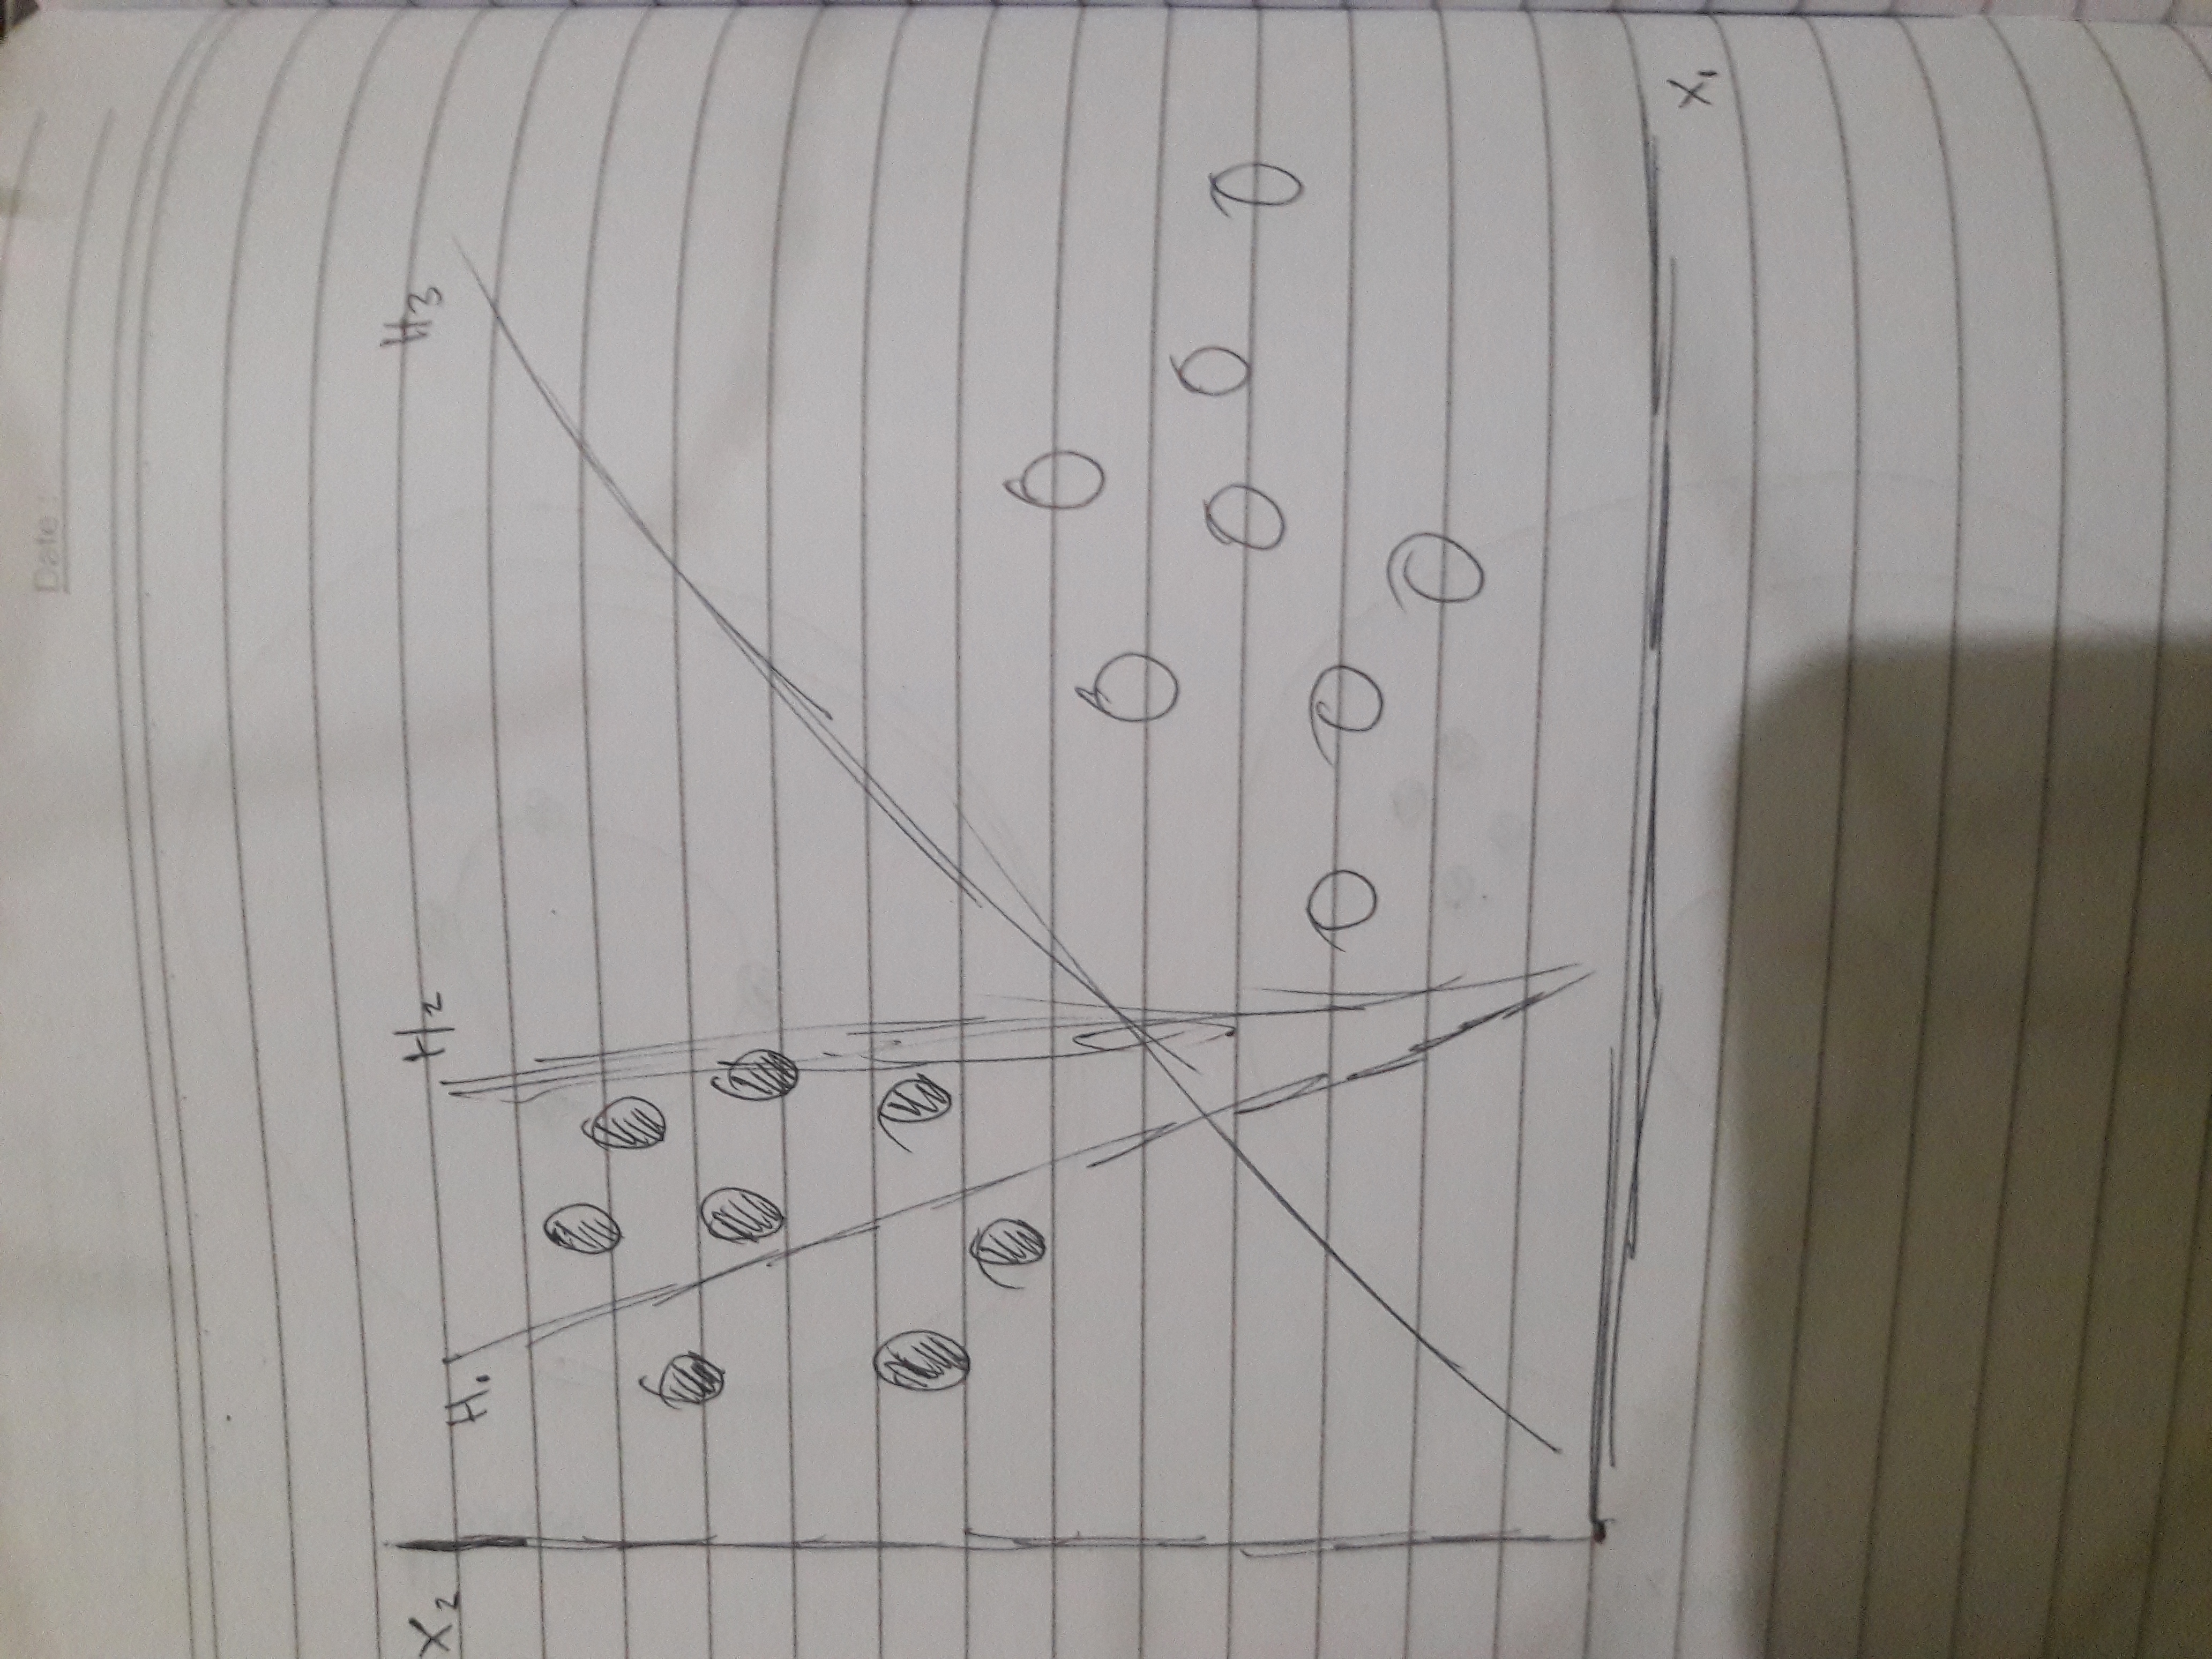
\includegraphics[width=4cm]{figures/1174056/2/1.jpg}
		\centering
		\caption{classication}
	\end{figure}
	Klasifikasi biner atau binomial adalah sebuah tugas untuk mengklasifikasikan elemen-elemen dari himpunan yang diberikan ke dalam dua kelompok (memprediksi kelompok mana yang masing-masing dimiliki) berdasarkan aturan klasifikasi. 
	Konteks yang membutuhkan keputusan apakah suatu item memiliki sifat kualitatif atau tidak, beberapa karakteristik tertentu, atau beberapa klasifikasi biner khas meliputi
	\begin{itemize}
		\item Tes medis untuk menentukan apakah pasien memiliki penyakit tertentu atau tidak - properti klasifikasi adalah keberadaan penyakit.
		\item Metode uji "lulus atau gagal" atau kontrol kualitas di pabrik, yaitu memutuskan apakah suatu spesifikasi telah atau belum terpenuhi - klasifikasi Go / no go.
		\item Pengambilan informasi, yaitu memutuskan apakah suatu halaman atau artikel harus dalam hasil pencarian atau tidak - properti klasifikasi adalah relevansi artikel, atau kegunaannya bagi pengguna.
	\end{itemize}
	\hfill\break
	Klasifikasi biner adalah dikotomisasi yang diterapkan untuk tujuan praktis, dan dalam banyak masalah klasifikasi biner praktis, 
	kedua kelompok 2 tidak simetris - daripada akurasi keseluruhan, proporsi relatif dari berbagai jenis kesalahan yang menarik. 
	Misalnya, dalam pengujian medis, false positive (mendeteksi penyakit ketika tidak ada) dianggap berbeda dari false negative 
	(tidak mendeteksi penyakit ketika hadir).
	\item Jelaskan apa itu supervised learning dan unsupervised learning dan clustering dengan ilustrasi gambar sendiri.
	\hfill\break
	\begin{figure}[H]
		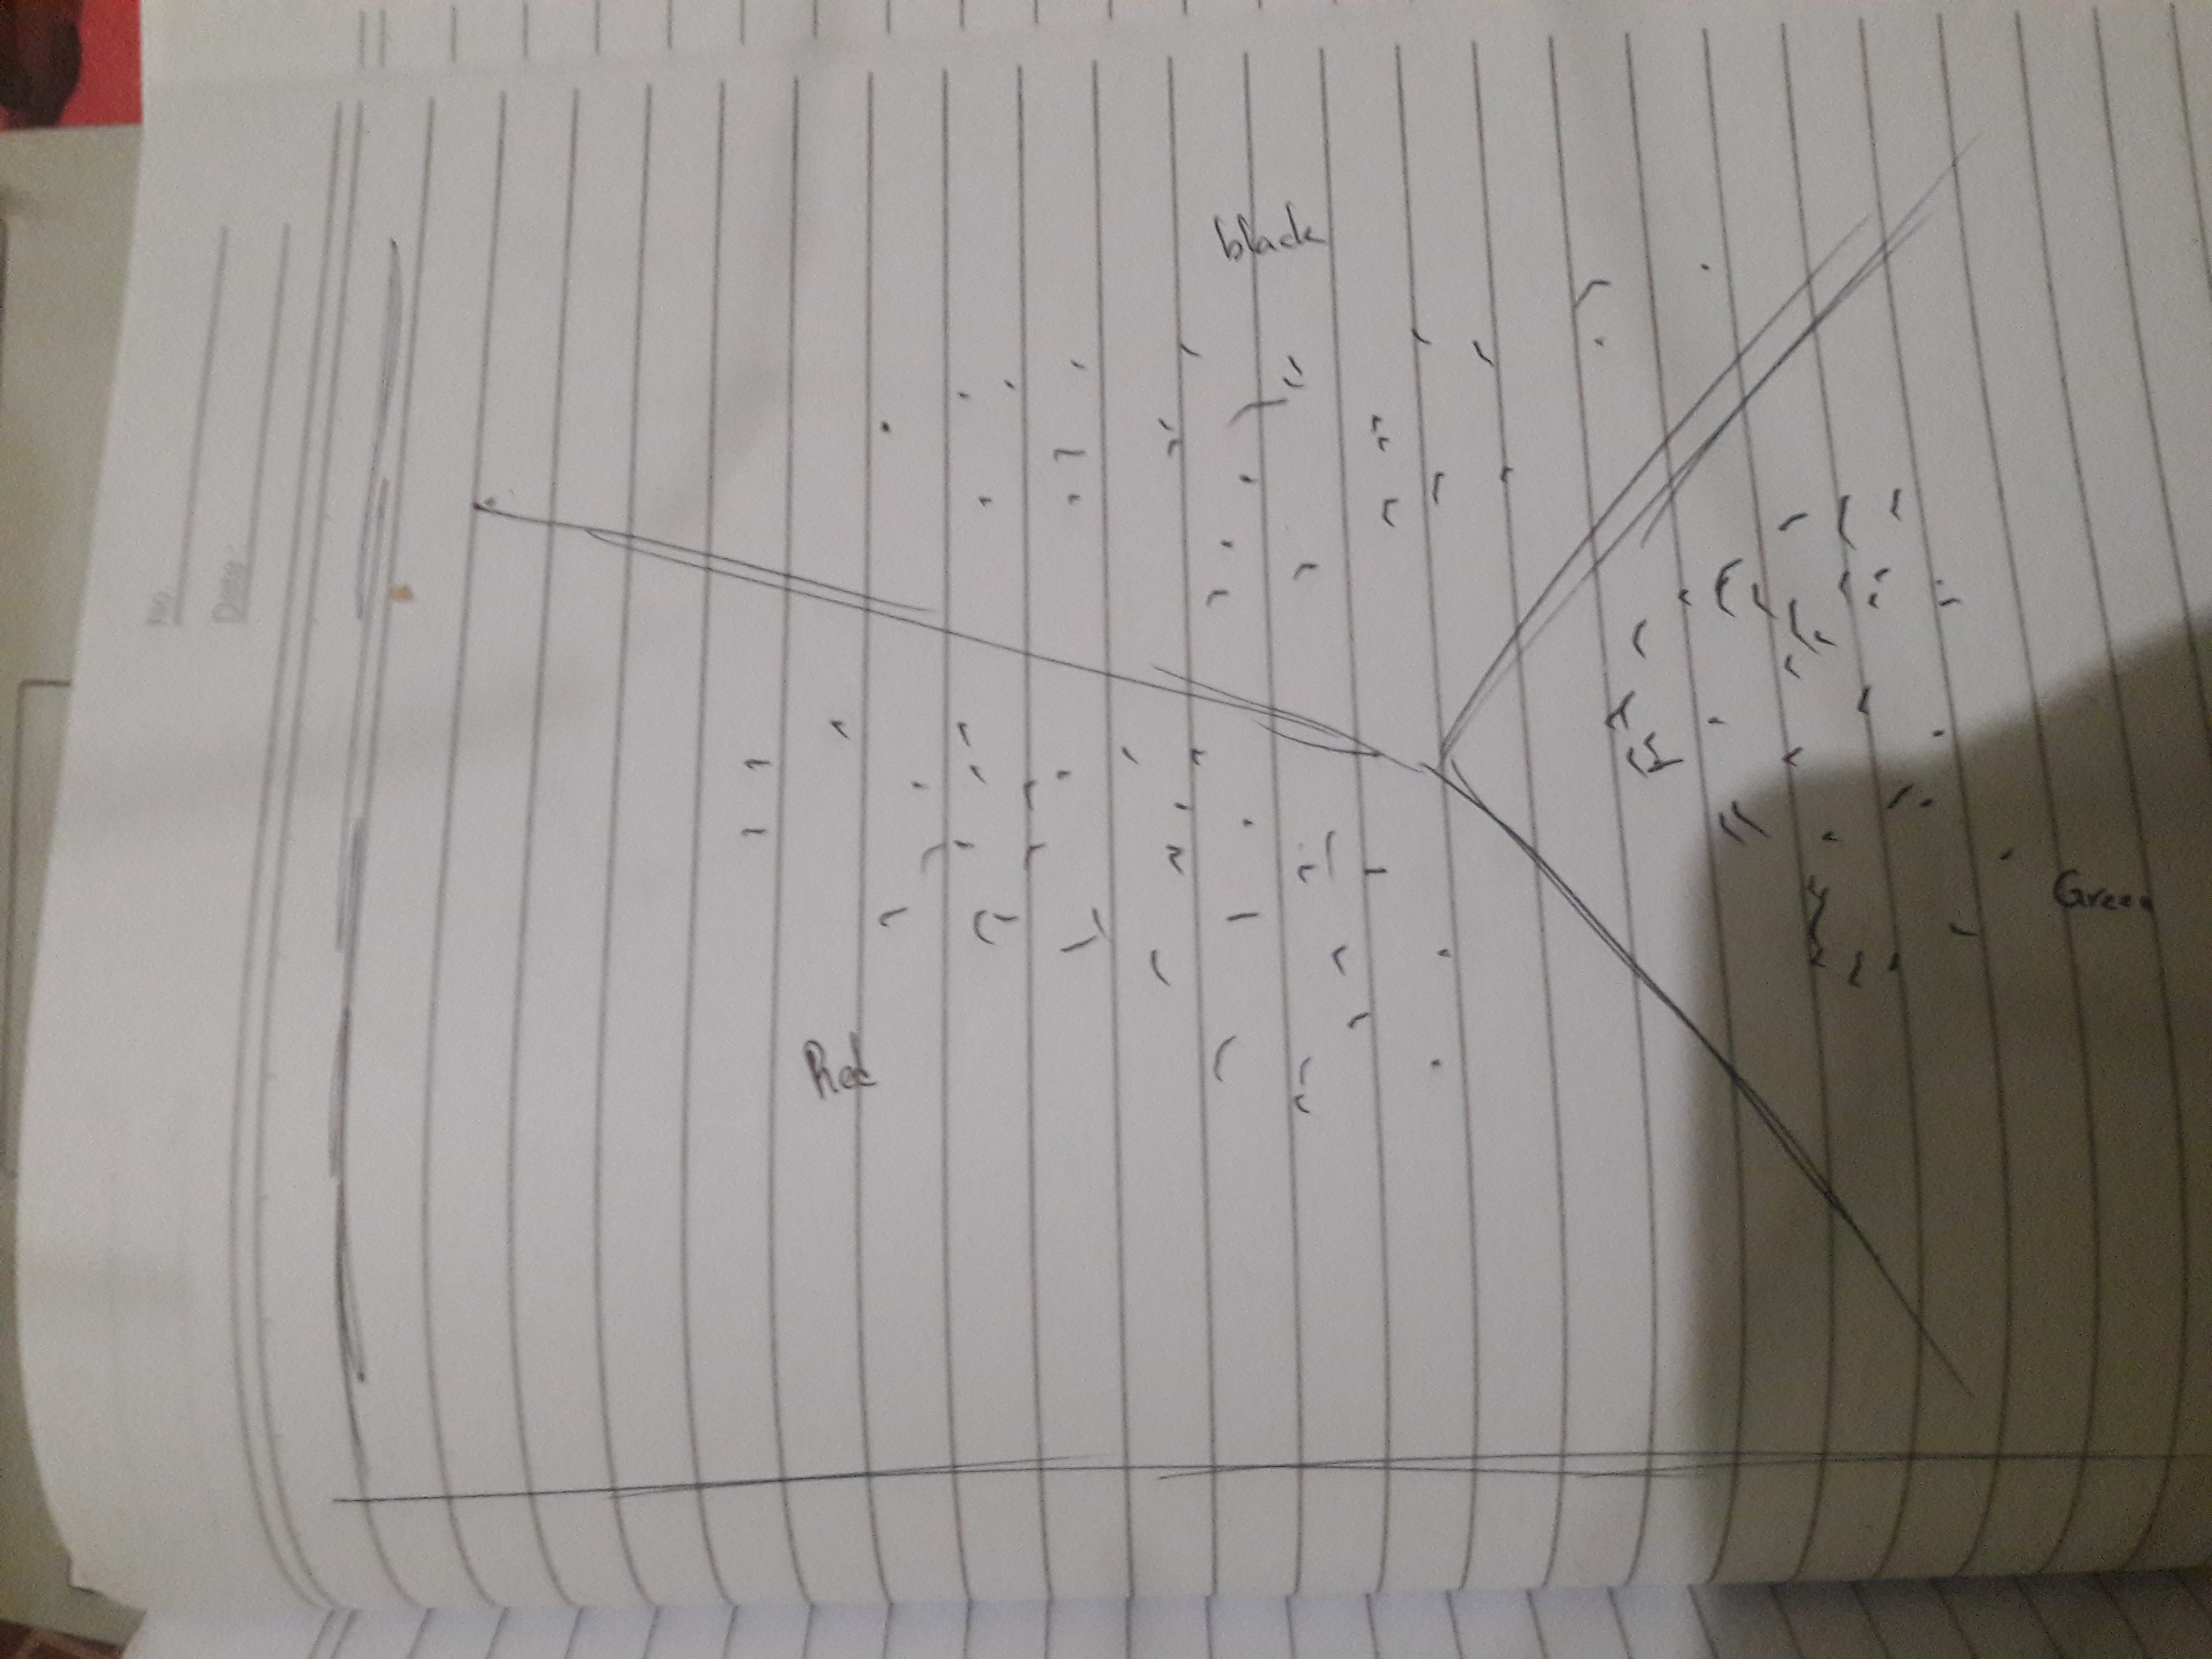
\includegraphics[width=4cm]{figures/1174056/2/clustering.jpg}
		\centering
		\caption{Clustering}
	\end{figure}
	\hfill\break
	clustering merupakan peroses mengklasifikasikan yang berdasarkan suatu parameter dalam penentuannya contoh pada berat sayuran sayuran A memiliki berat 100 gr dan sayuran B memiliki berat 120 gr yang berarti berat sayuran dibagi dua parameter yaitu lebih kecil samadengan 100 gram dan lebih besar dari gram contoh pada gambar.\par
		\begin{figure}[H]
		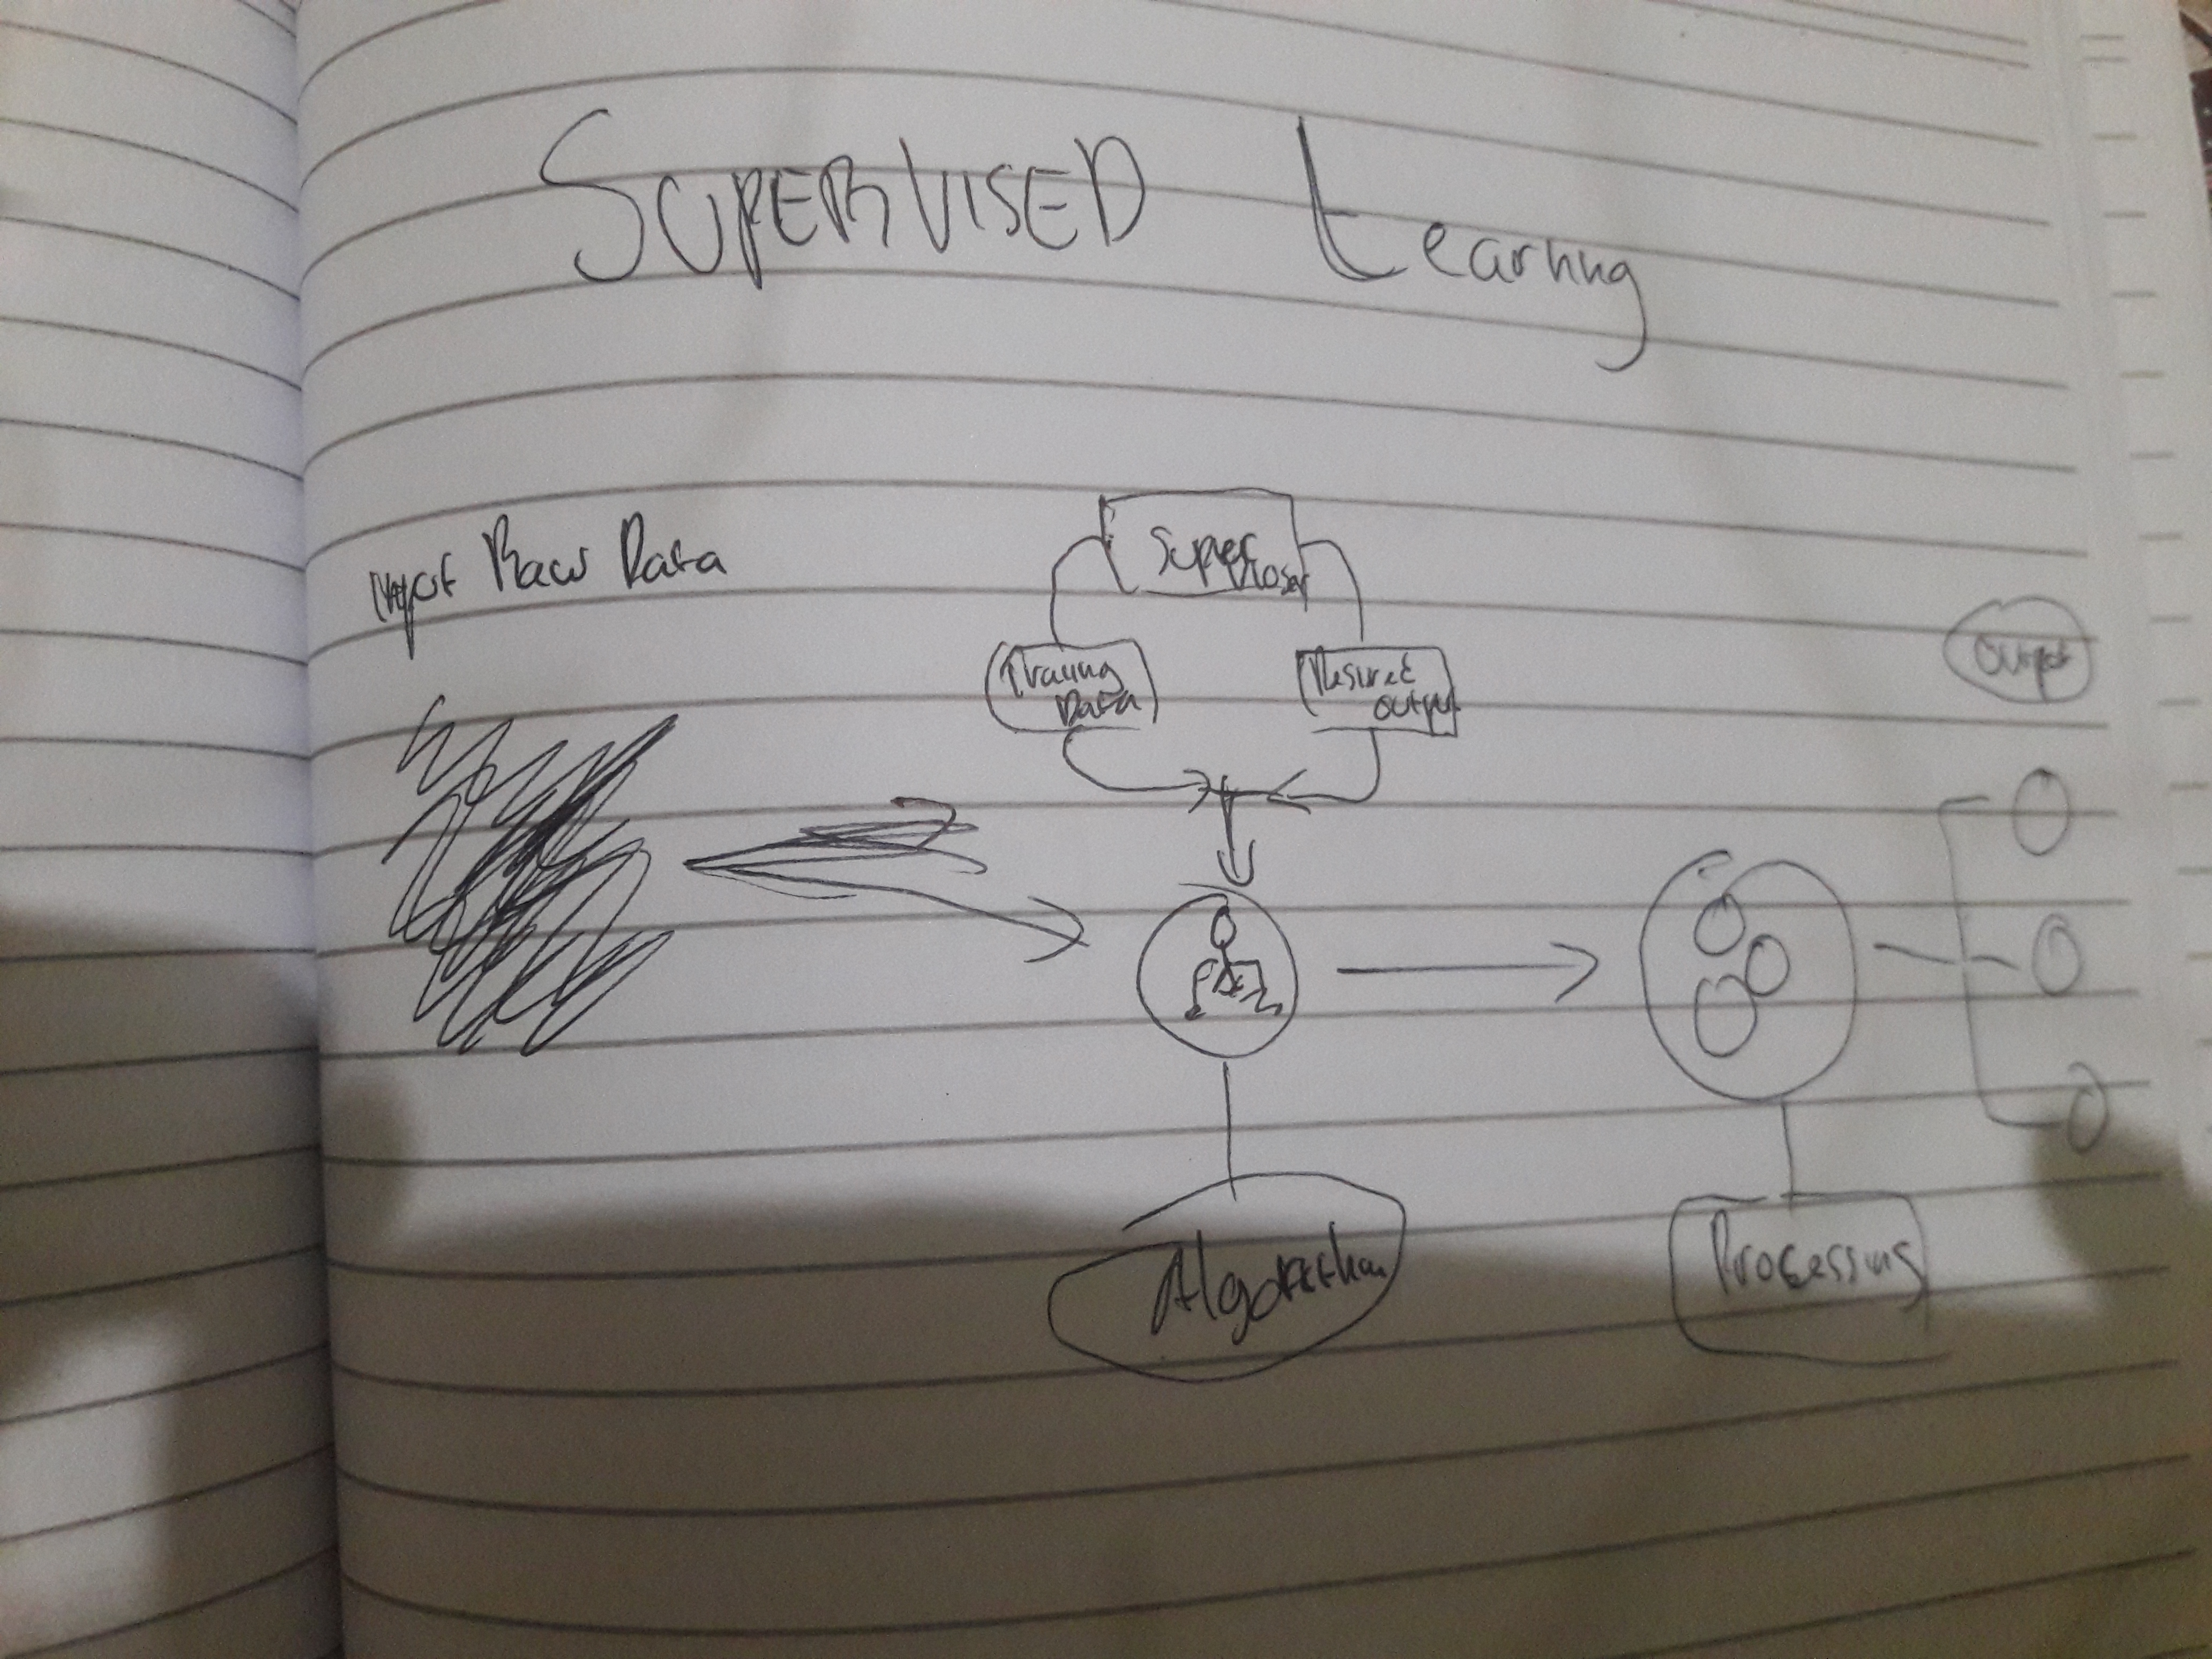
\includegraphics[width=4cm]{figures/1174056/2/supervised.png}
		\centering
		\caption{Supervised Learning}
	\end{figure}
	\hfill\break
	supervised learning adalah cara untuk mengklasifikasikan suatu objek atau data yang telah di tentukan kelas kelasnya contoh pada sayuran tumbuhan wortel termasuk yang mengandung vitamin A berarti tumbuhan wortel telah di kategorikan kedalam sayuran yang mengandung vitamin A. sedangkan kangkung mengandung zat besi yang berarti tumbuhan kangkung telah di kategorikan kedalam sayuran yang mengandung zat besi untuk lebih jelasnya dapat dilihat pada gambar.\par
		\begin{figure}[H]
		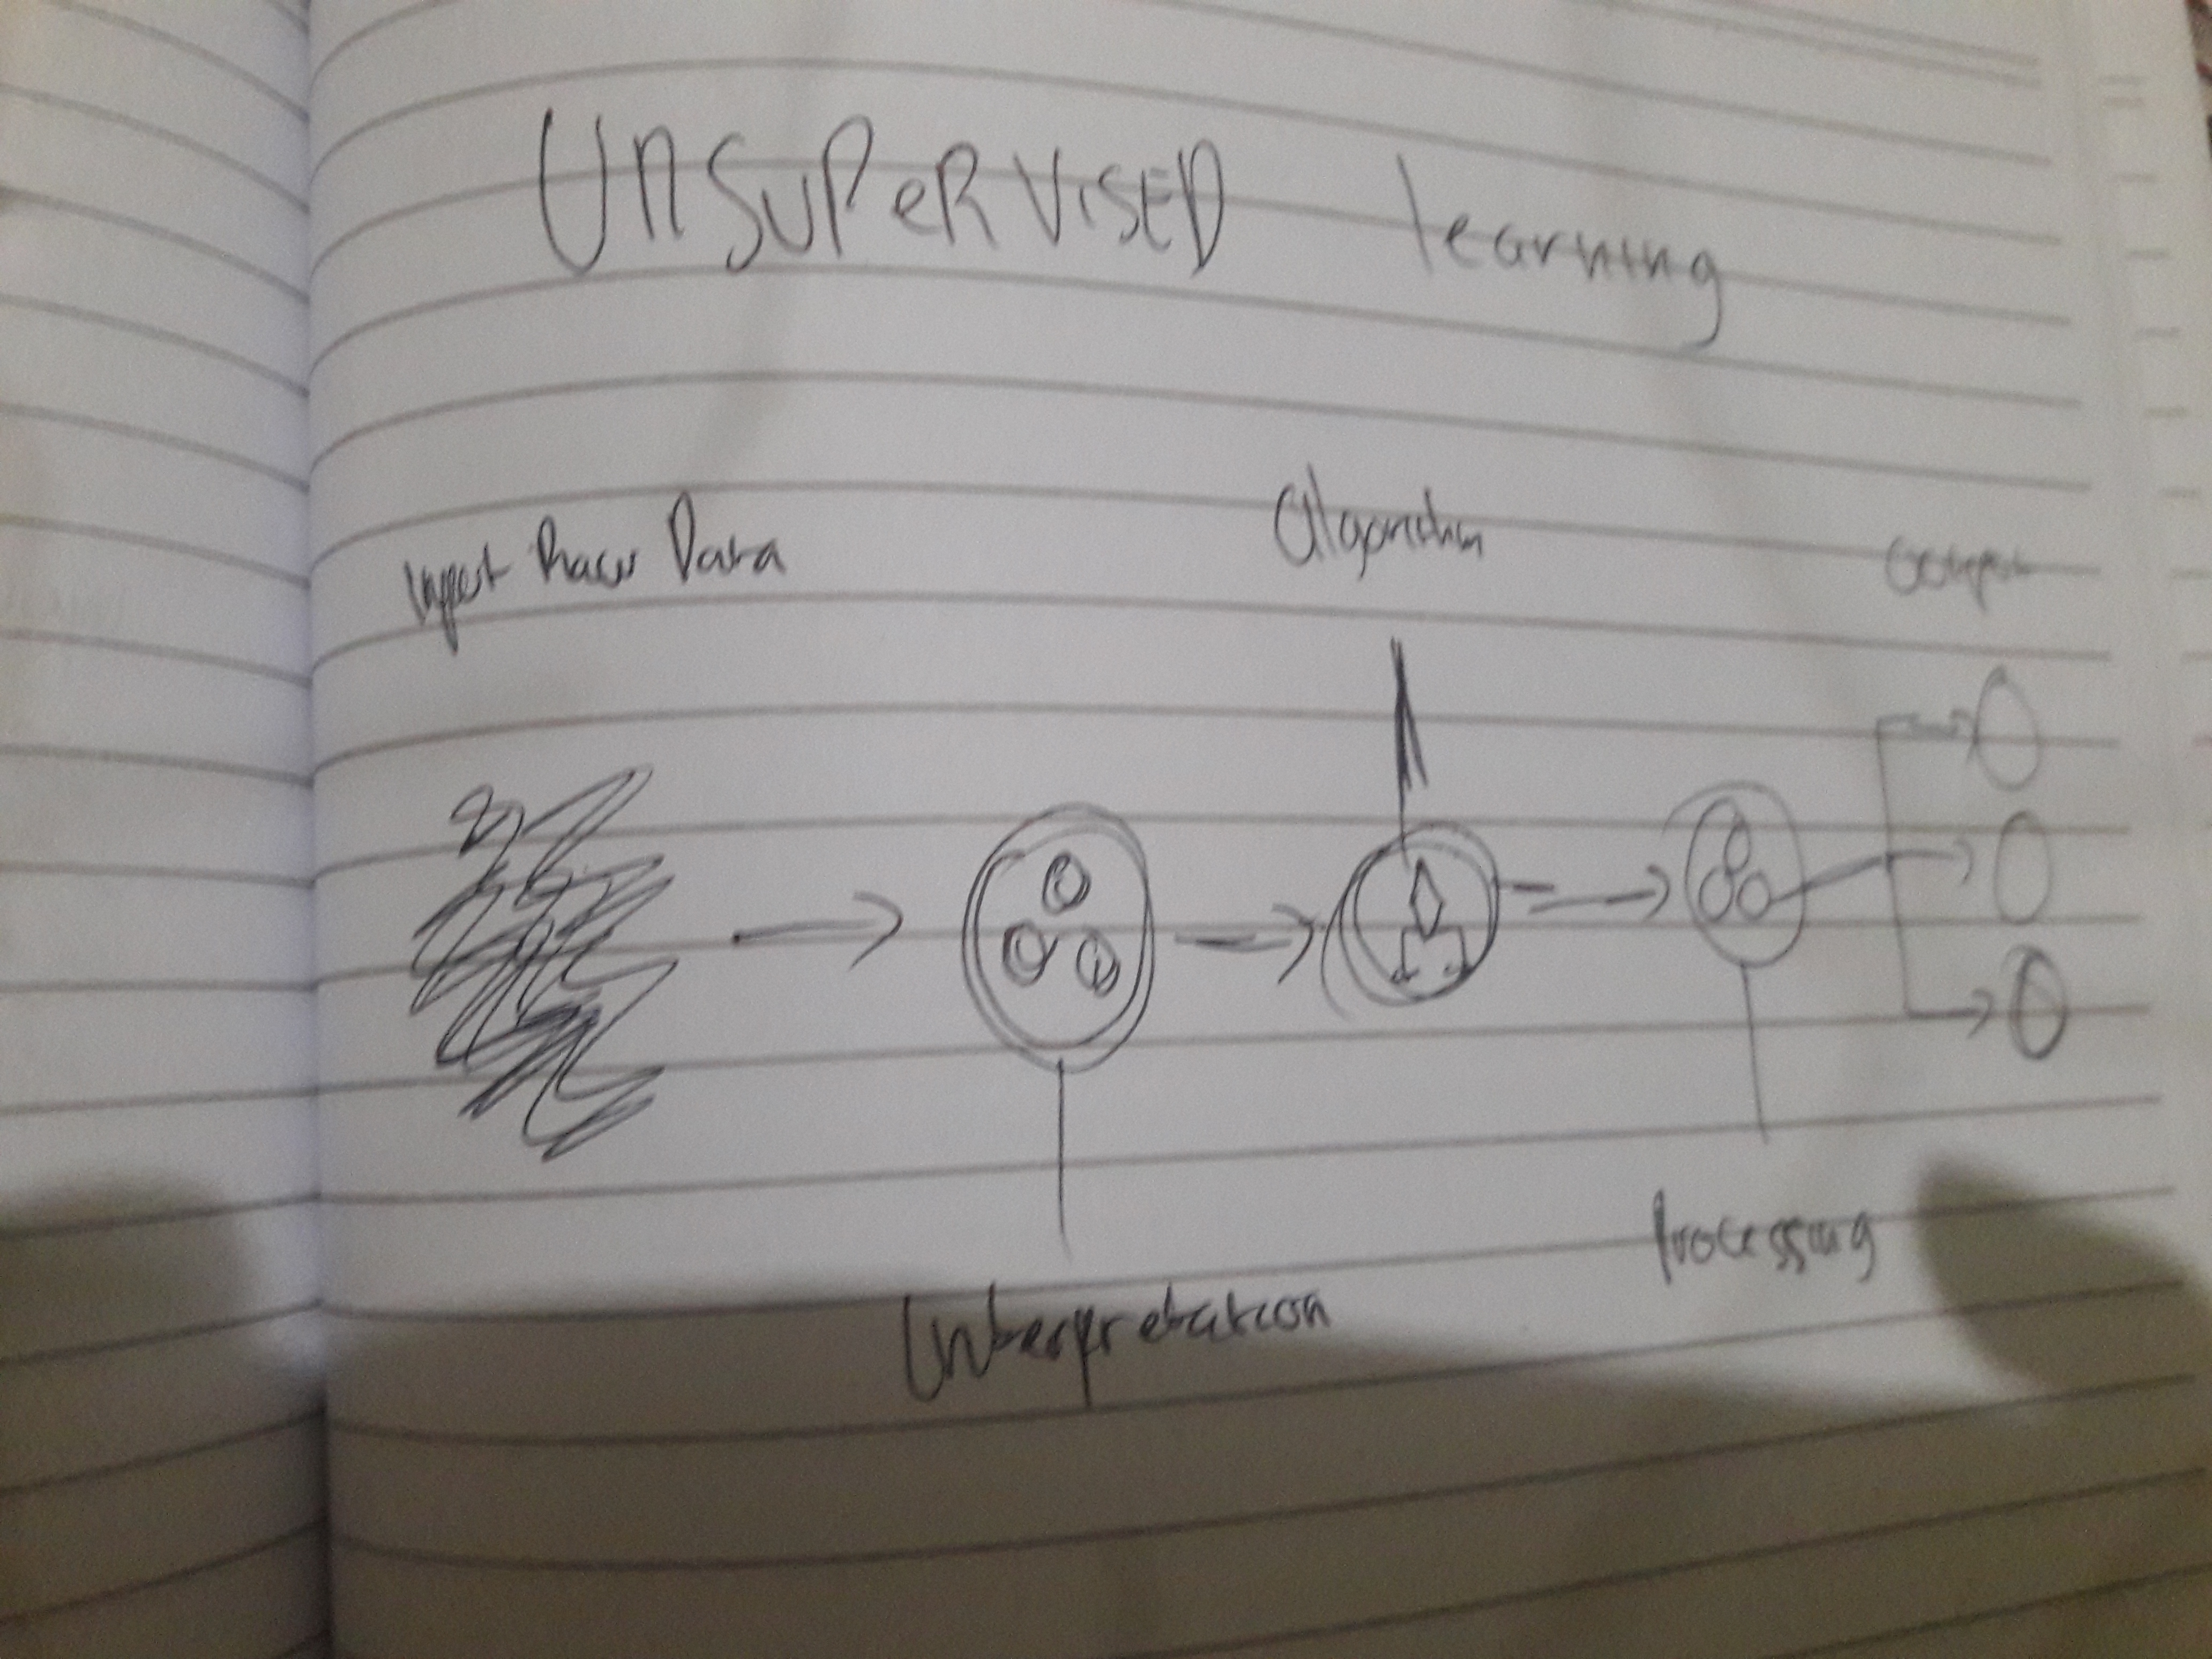
\includegraphics[width=4cm]{figures/1174056/2/unsupervised.png}
		\centering
		\caption{Unsupervised Learning}
	\end{figure}
	\hfill\break
	unsupervised learning merupakan cara untuk mengklasifikasi tanpa adanya kelas untuk menentukan jenisnya contoh sayuran berarti semua objek yang memiliki ciri ciri sayuran di kategorikan kedalam sayuran untuk lebih jelasnya dapat dilihat pada gambar.\par
	\item Jelaskan apa itu evaluasi dan akurasi dari buku dan disertai ilustrasi contoh dengan gambar sendiri
	\hfill\break
	\begin{figure}[H]
		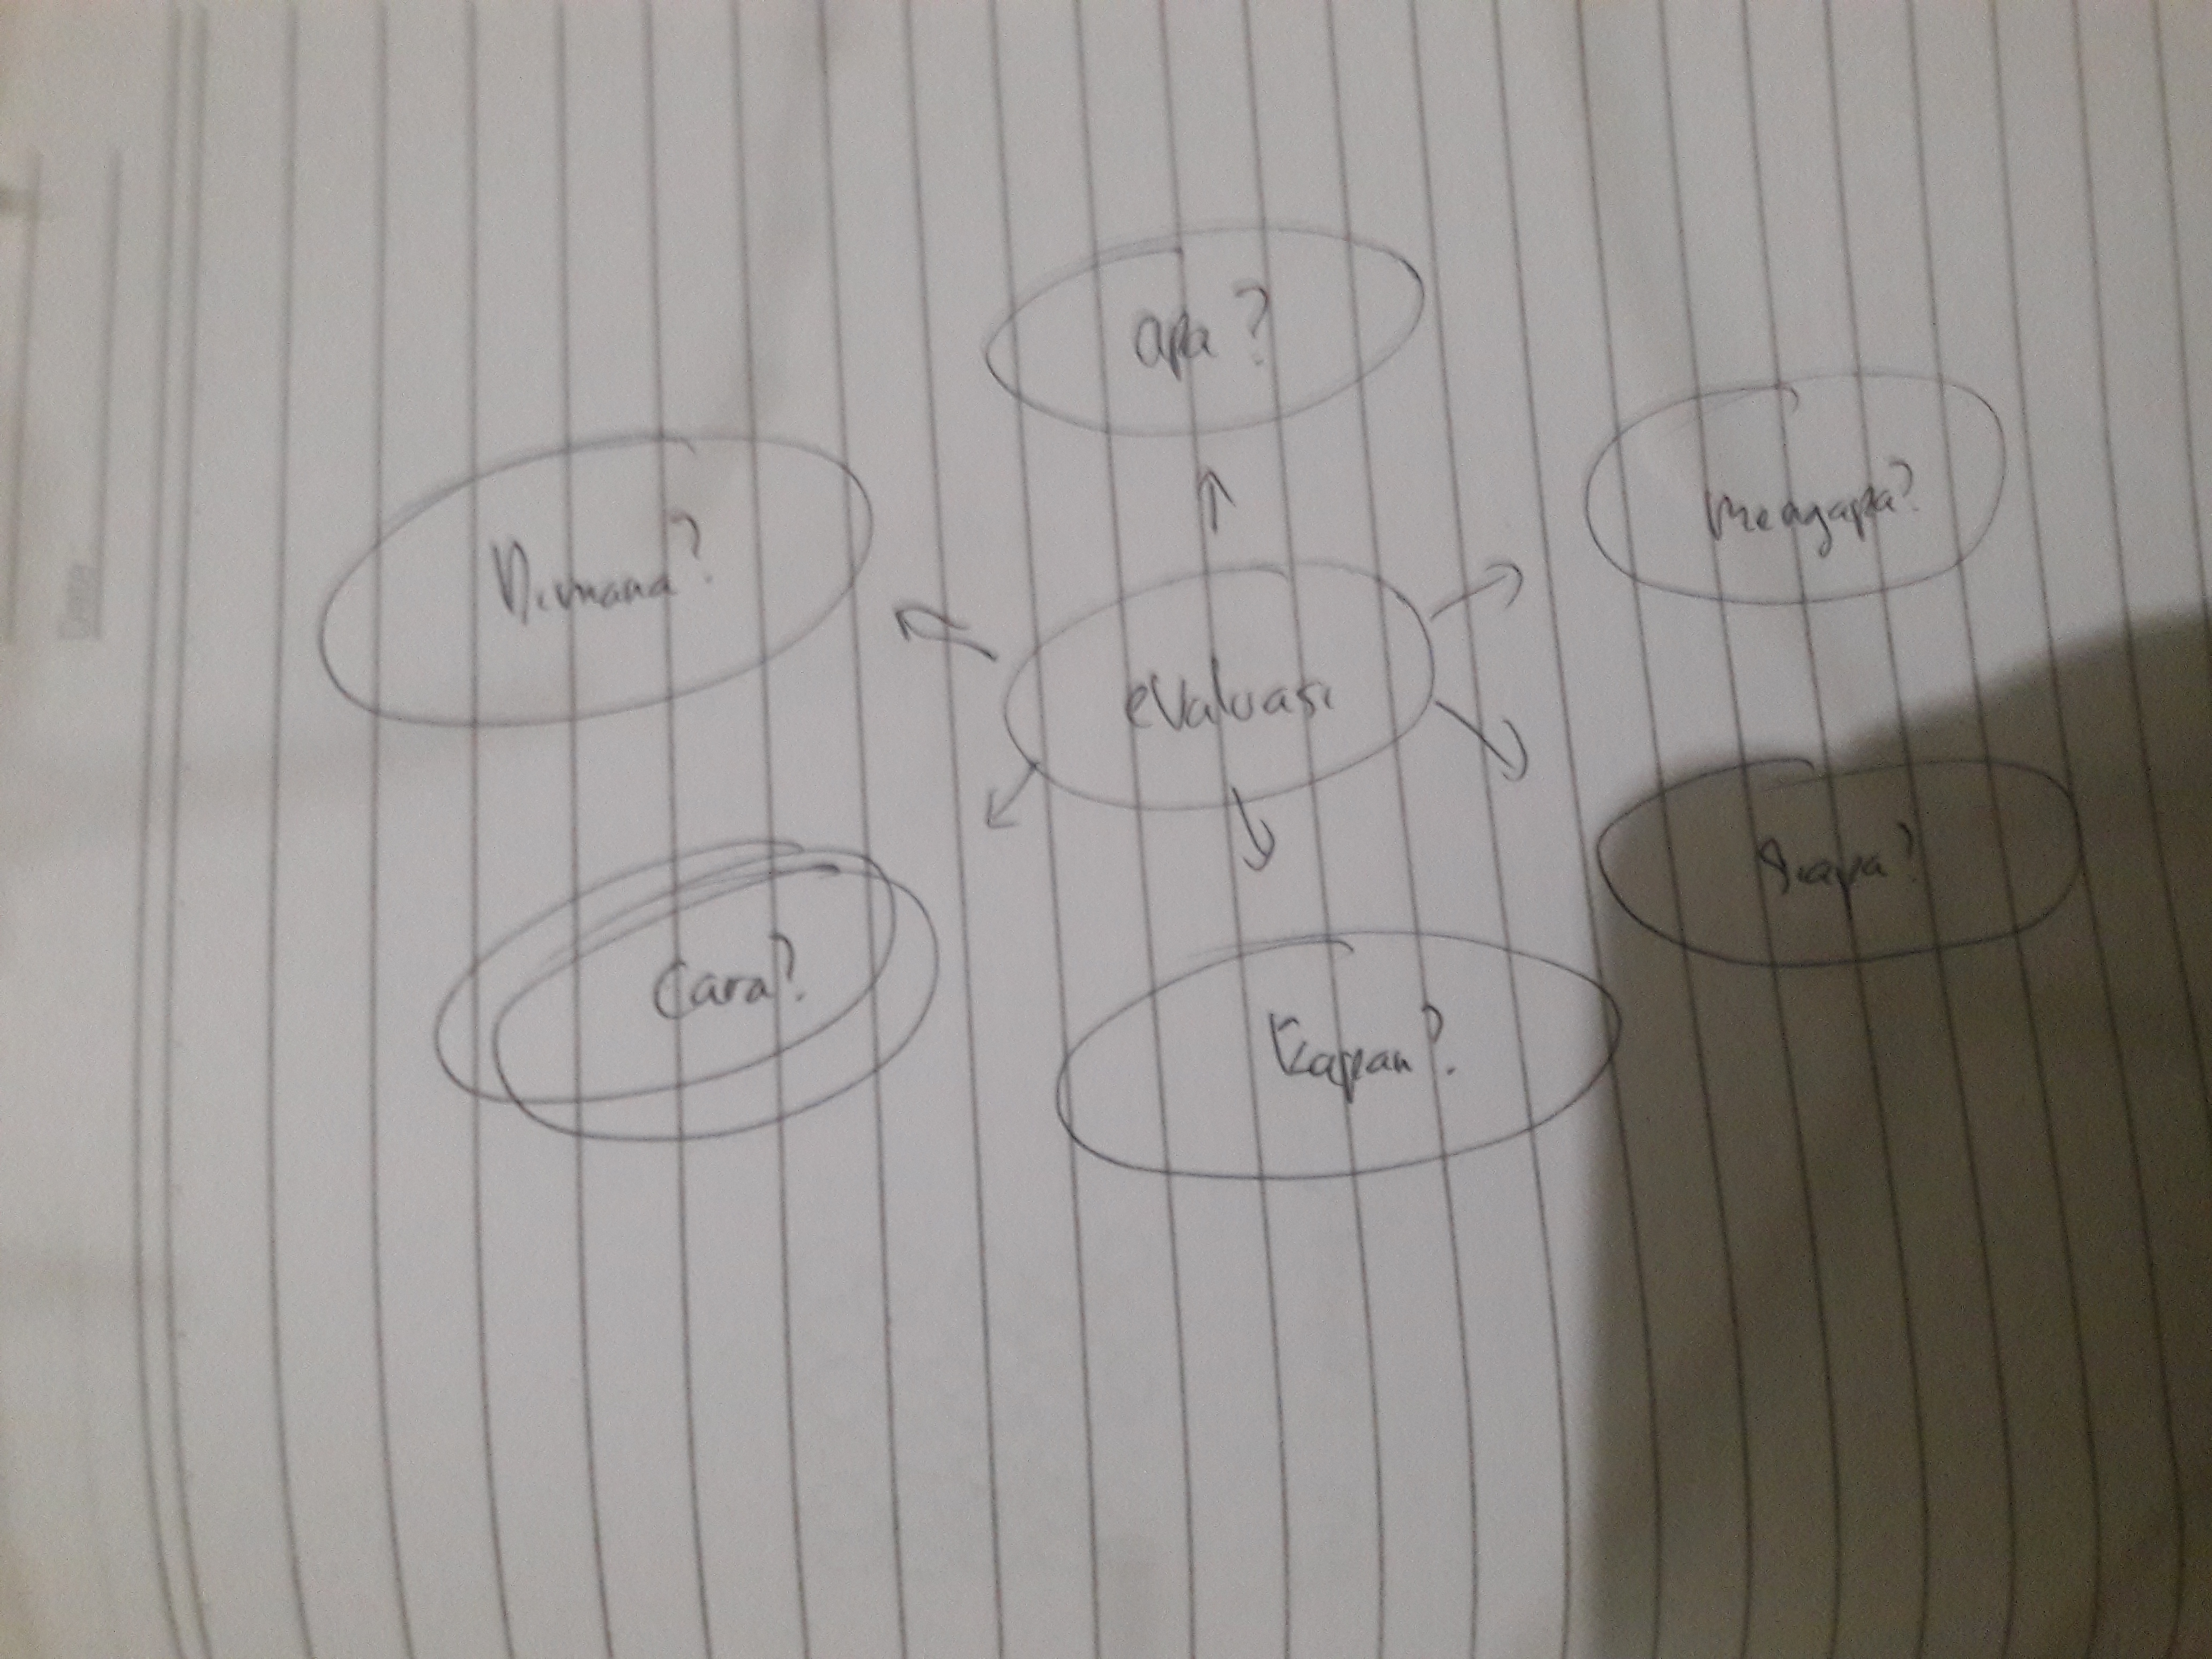
\includegraphics[width=4cm]{figures/1174056/2/Evaluasi.jpg}
		\centering
		\caption{Evaluasi}
	\end{figure}
	\hfill\break
	Evaluasi didefinisikan sebagai penilaian atau penilaian. Nurkancana (1983) menyatakan bahwa evaluasi adalah kegiatan yang dilakukan berkaitan dengan proses 
	penentuan nilai suatu masalah. Sedangkan Raka Joni (1975) menjelaskan evaluasi proses untuk menilai suatu barang, benda atau variasi dengan pertimbangan berbagai 
	faktor yang kemudian disebut Penilaian Nilai.
	\begin{figure}[H]
		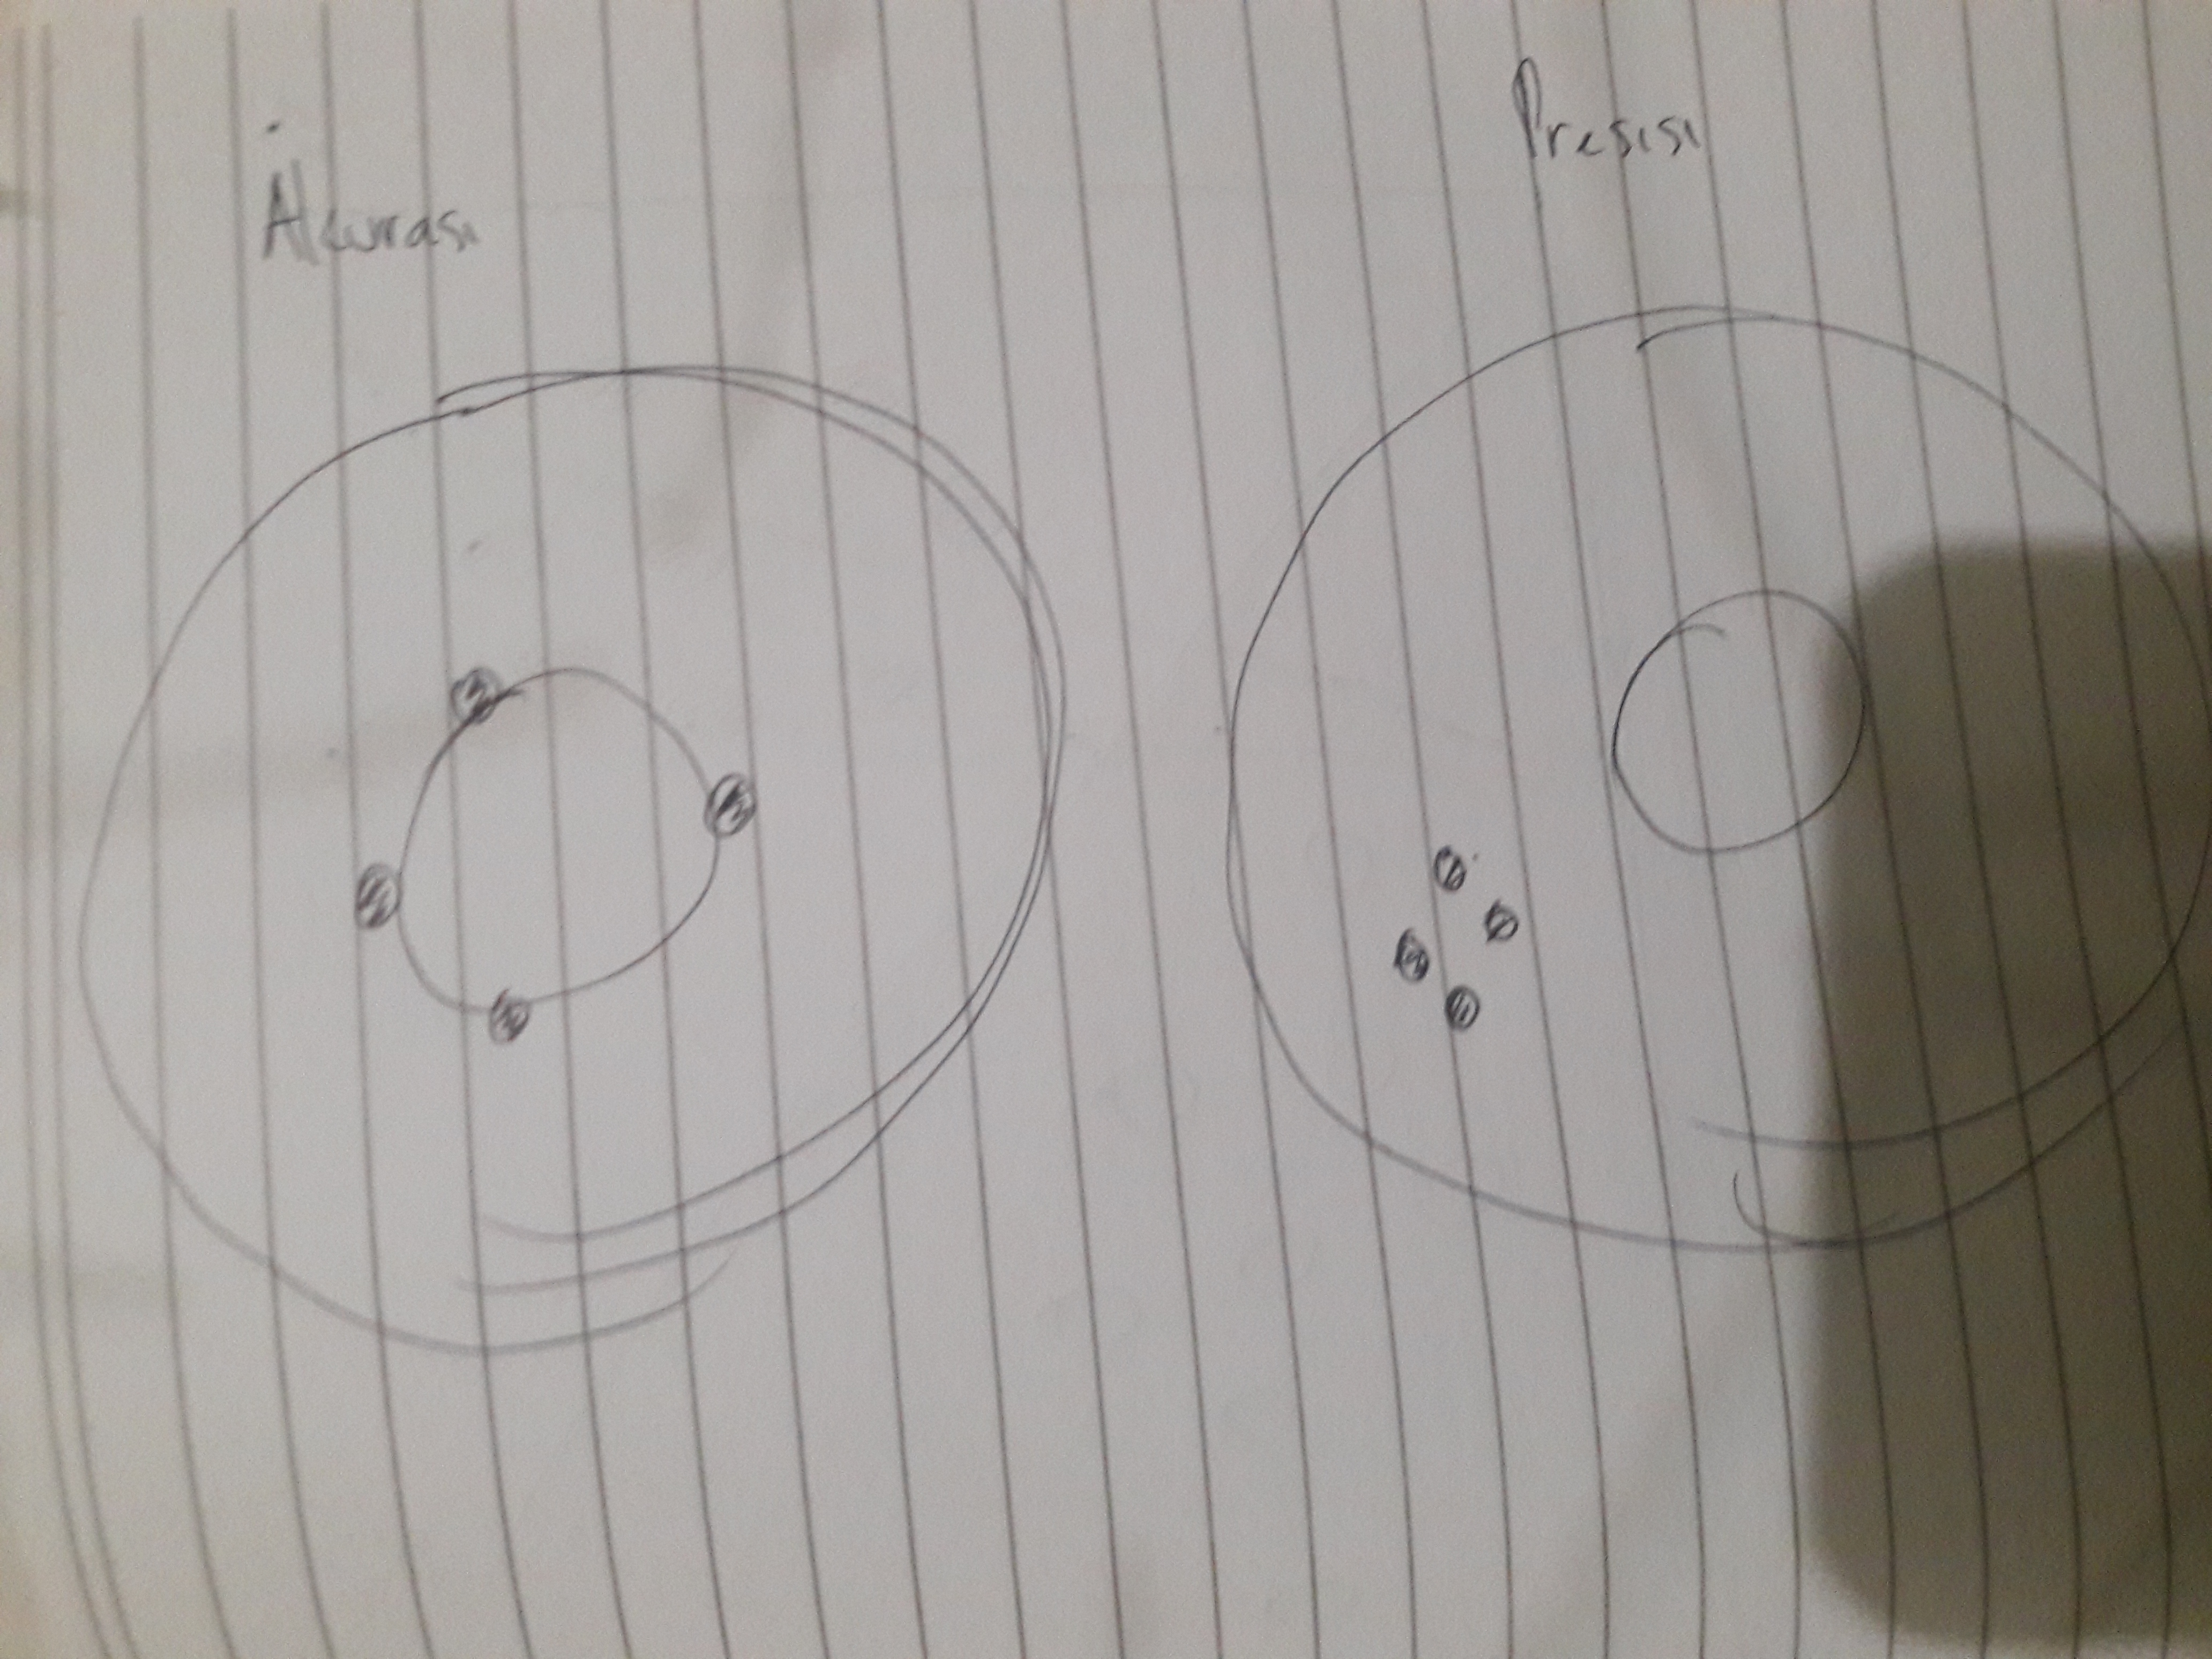
\includegraphics[width=4cm]{figures/1174056/2/akurasi.jpg}
		\centering
		\caption{Akurasi}
	\end{figure}
	\hfill\break
	Akurasi adalah nilai yang dekat dengan nilai aktual. Contohnya mendekati panah target pusat (bullseye).
	\item Jelaskan bagaimana cara membuat dan membaca confusion matrix, buat confusion matrix buatan sendiri.
	\hfill\break
	\begin{figure}[H]
		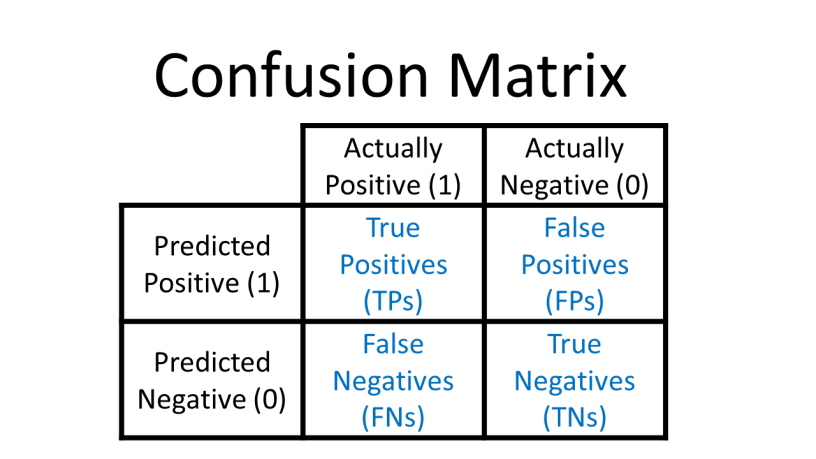
\includegraphics[width=4cm]{figures/1174056/2/confusionmatrix.png}
		\centering
		\caption{Confusionmatrix}
	\end{figure}
	\hfill\break
	\item Jelaskan bagaimana K-fold cross validation bekerja dengan gambar ilustrasi contoh buatan sendiri.
	\hfill\break
	\begin{figure}[H]
		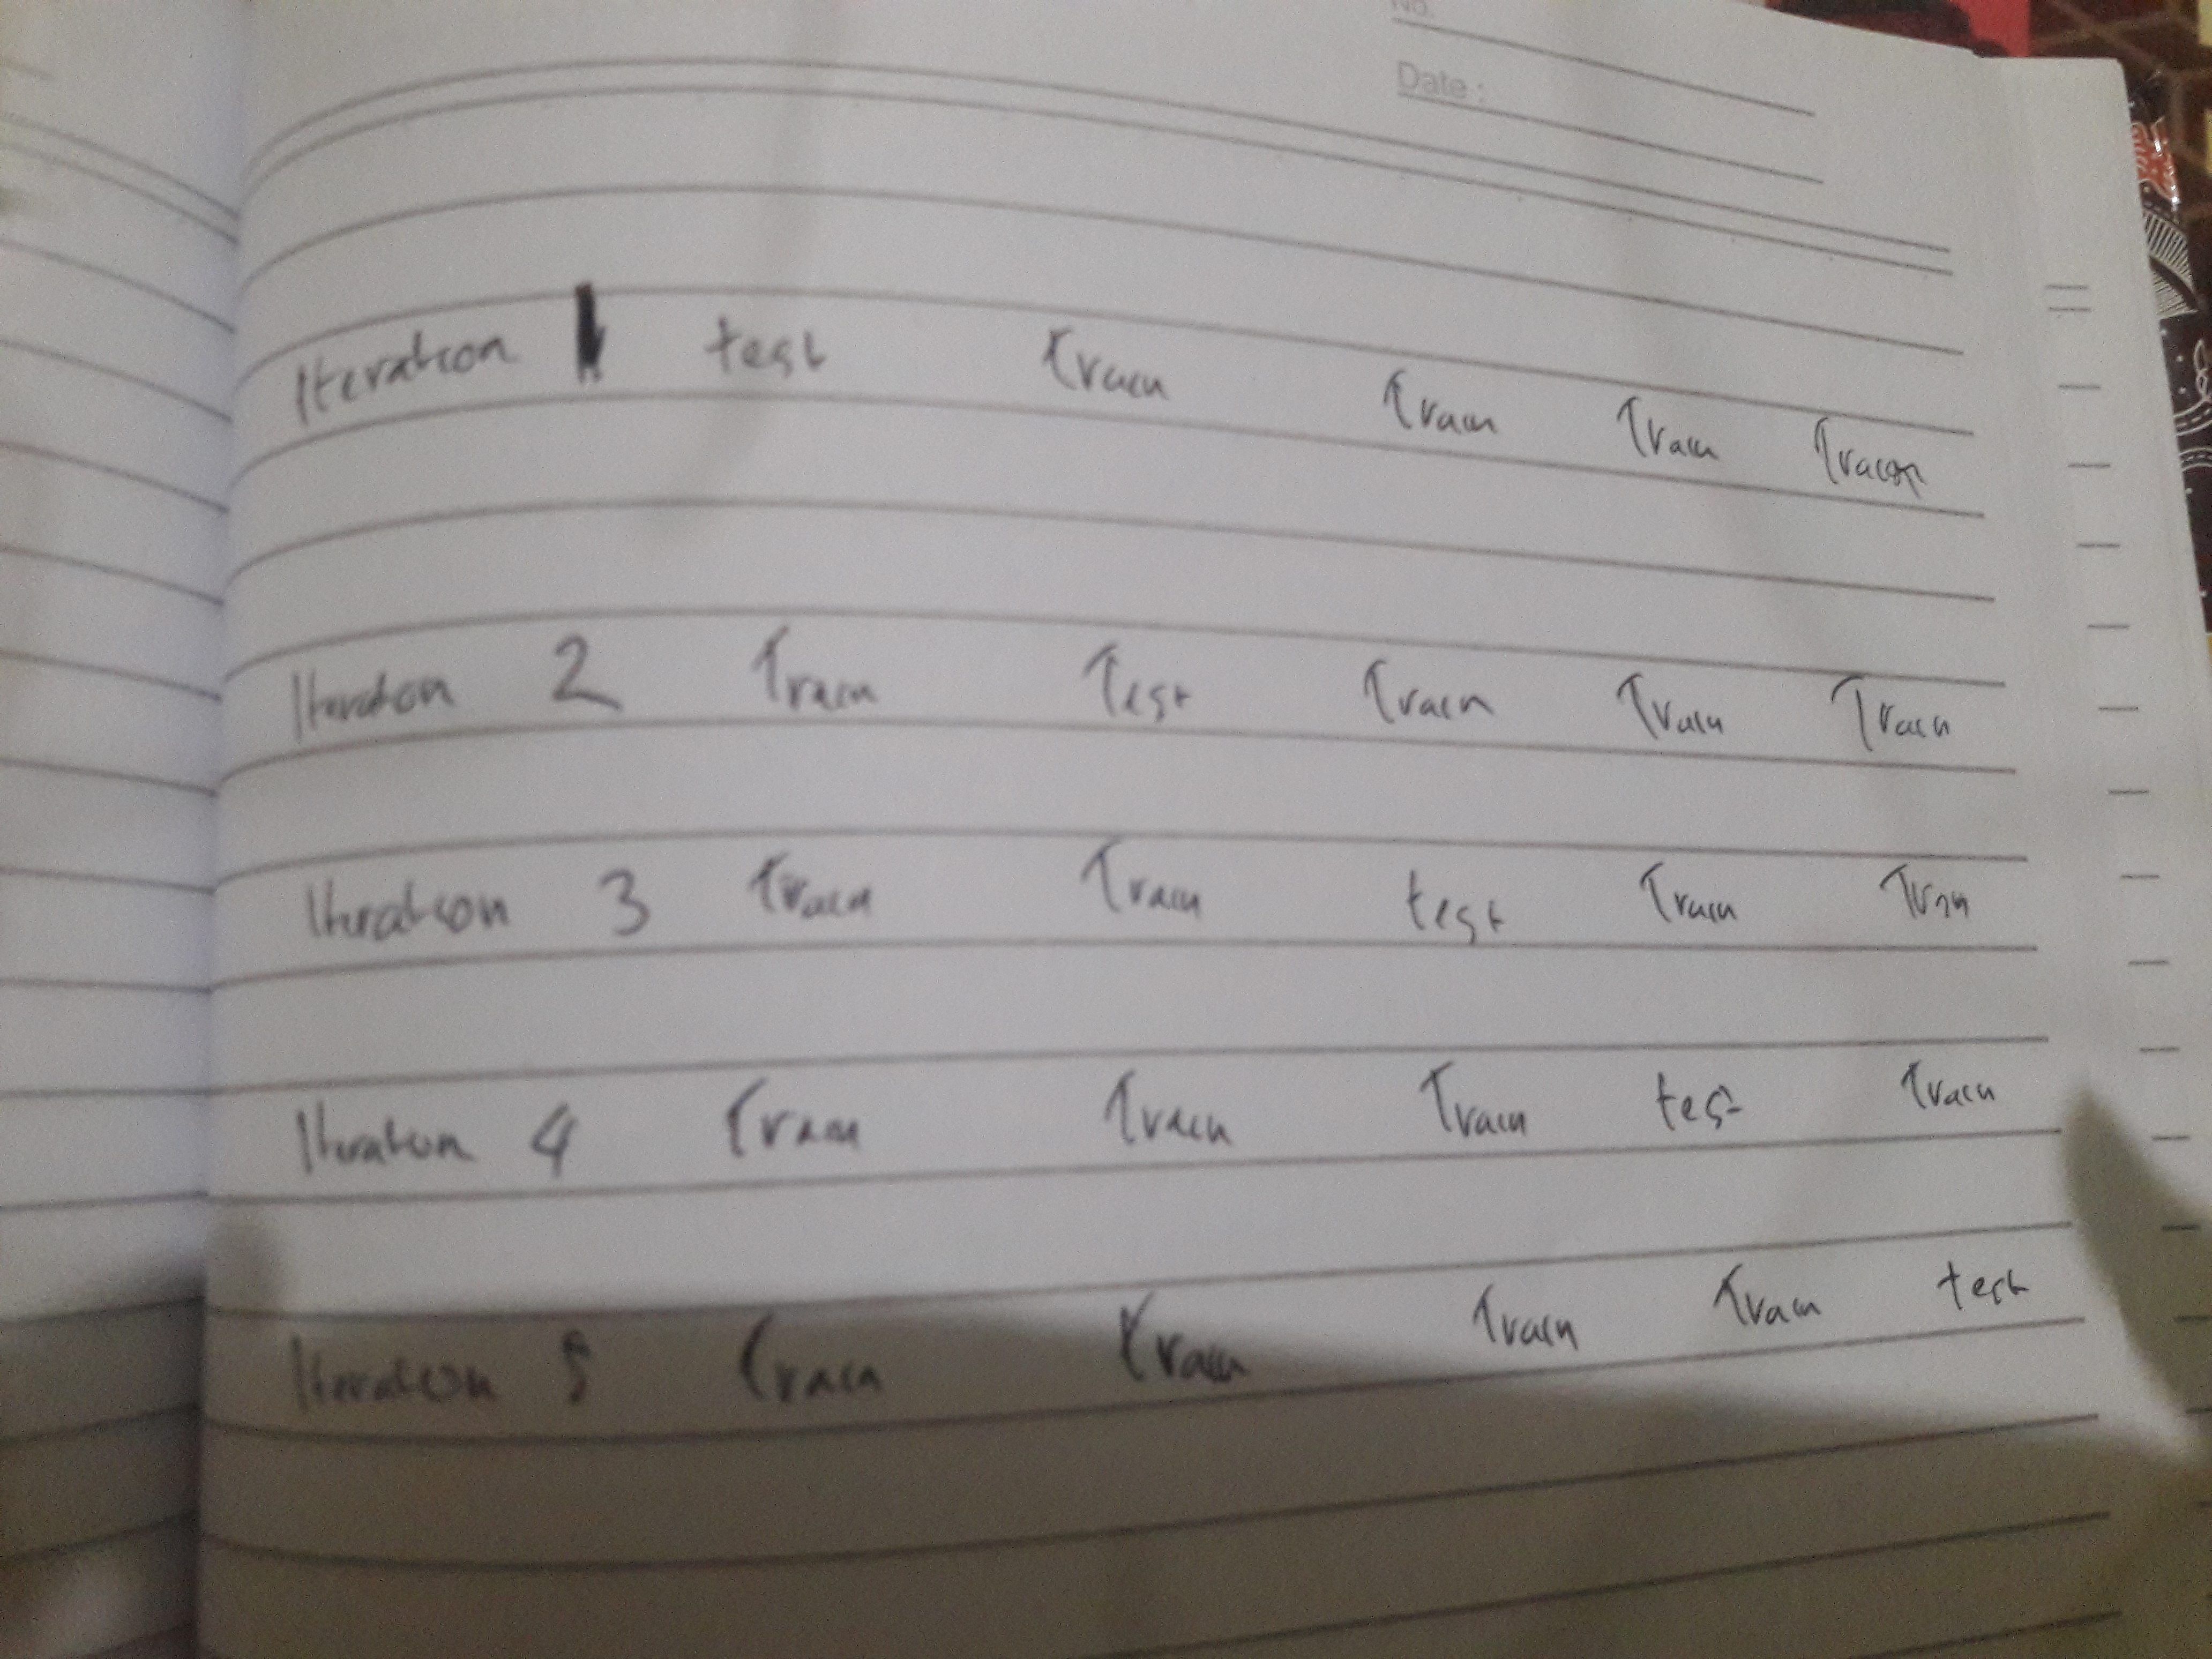
\includegraphics[width=4cm]{figures/1174056/2/kfold.png}
		\centering
		\caption{K-fold}
	\end{figure}
	\hfill\break
	K-fold cross validation adalah salah satu metode untuk mendapatkan kinerja classifier, 
	metode ini dapat digunakan dengan jumlah data yang terbatas (tidak banyak contoh).
	Cara kerja K-fold cross validation adalah sebagai berikut
	\begin{enumerate}
		\item Total instance dibagi menjadi N bagian.
		\item Fold-1 adalah ketika bagian 1 menjadi data uji (data pengujian) dan sisanya menjadi data pelatihan (data pelatihan).
		\hfill\break
		Selanjutnya, hitung keakuratan berdasarkan porsi data. Perhitungan akurasi menggunakan persamaan berikut:
		Akurasi = sigma data uji benar klasifikasi sigma total data uji x 100%%
		\item Fold ke-2 adalah ketika bagian ke-2 menjadi data uji (data pengujian) dan sisanya menjadi data pelatihan (data pelatihan).
		\hfill\break
		Selanjutnya, hitung keakuratan berdasarkan porsi data.4. 
		Demikian seterusnya hingga mencapai fold ke-K. 
		Hitung rata-rata akurasi dari K buah akurasi di atas. 
		Rata-rata akurasi ini menjadi akurasi final.
	\end{enumerate}
	\item Jelaskan apa itu decision tree dengan gambar ilustrasi contoh buatan sendiri.
	\hfill\break
	\begin{figure}[H]
		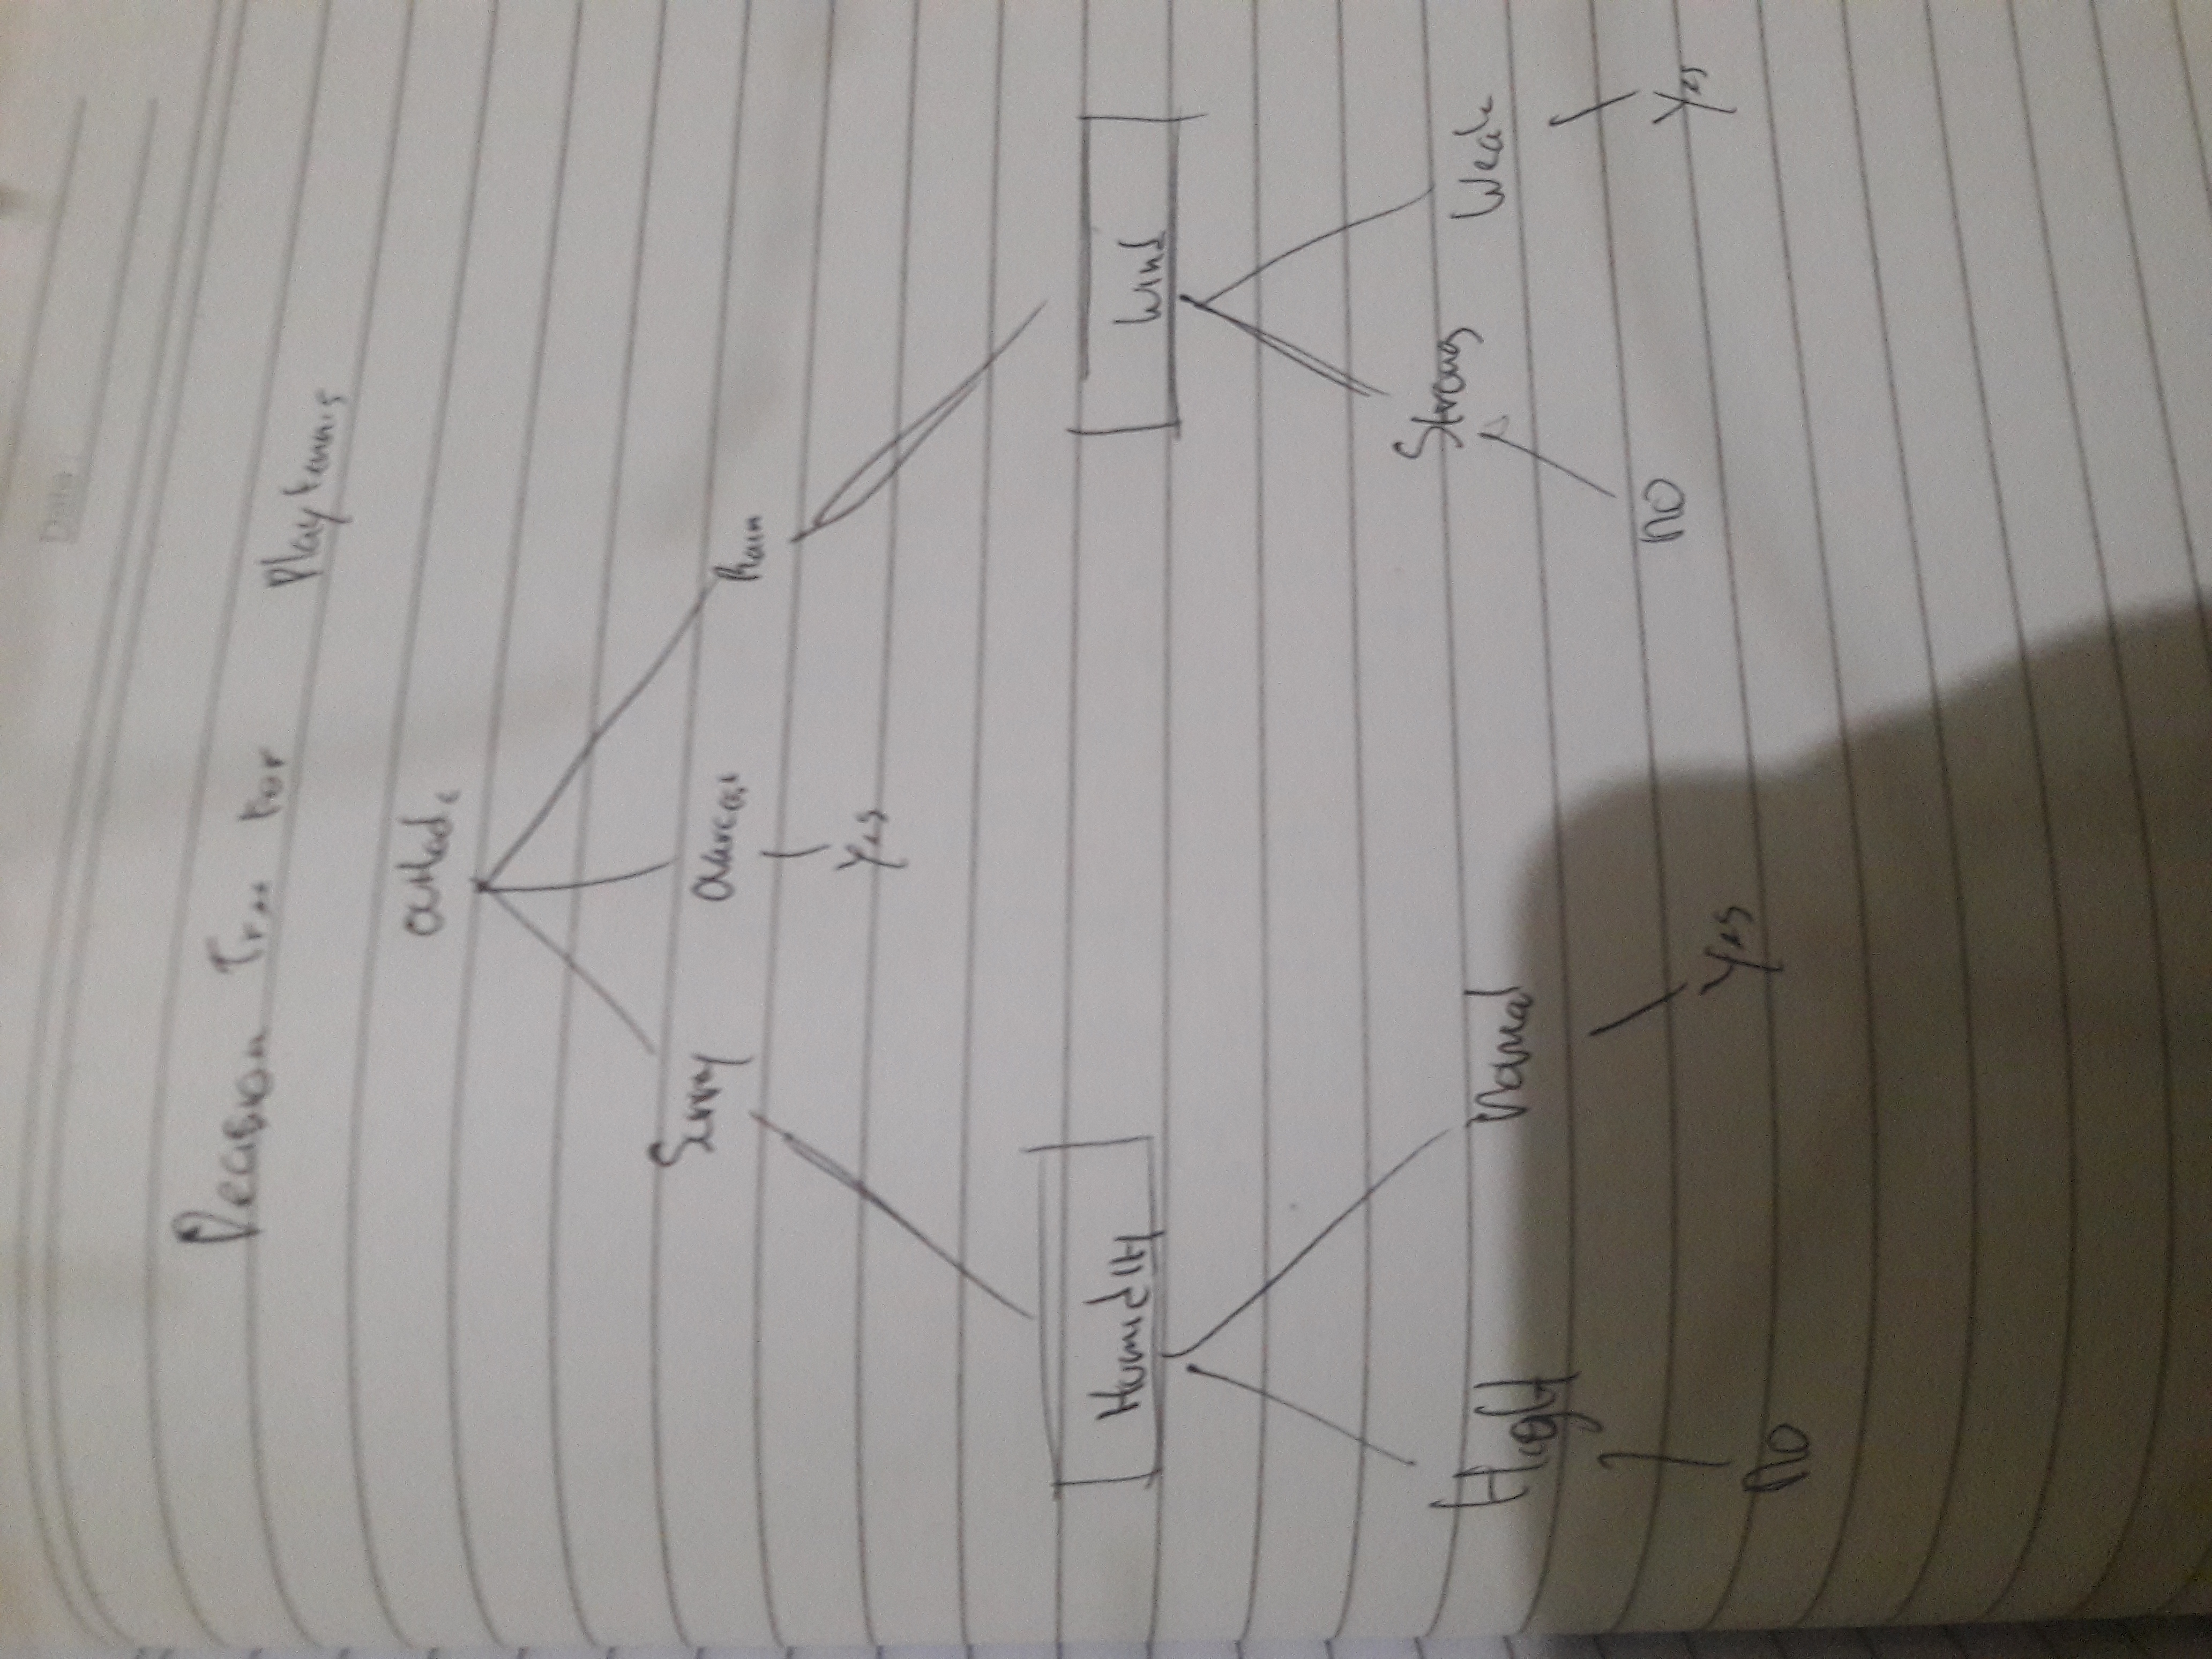
\includegraphics[width=4cm]{figures/1174056/2/Decisiontree.png}
		\centering
		\caption{Decision tree}
	\end{figure}
	\hfill\break
	Pohon keputusan adalah salah satu metode klasifikasi yang paling populer, karena mudah ditafsirkan oleh manusia. 
	Pohon keputusan adalah model prediksi yang menggunakan struktur pohon atau struktur hierarkis.
	Konsep pohon keputusan adalah mengubah data menjadi pohon keputusan dan aturan keputusan. 
	Manfaat utama menggunakan pohon keputusan adalah kemampuannya untuk memecah proses pengambilan keputusan yang menjadi lebih sederhana, 
	sehingga perolehan keputusan akan lebih baik menafsirkan solusi dari masalah.
	\item Jelaskan apa itu information gain dan entropi dengan gambar ilustrasi buatan sendiri
	\hfill\break
	\begin{figure}[H]
		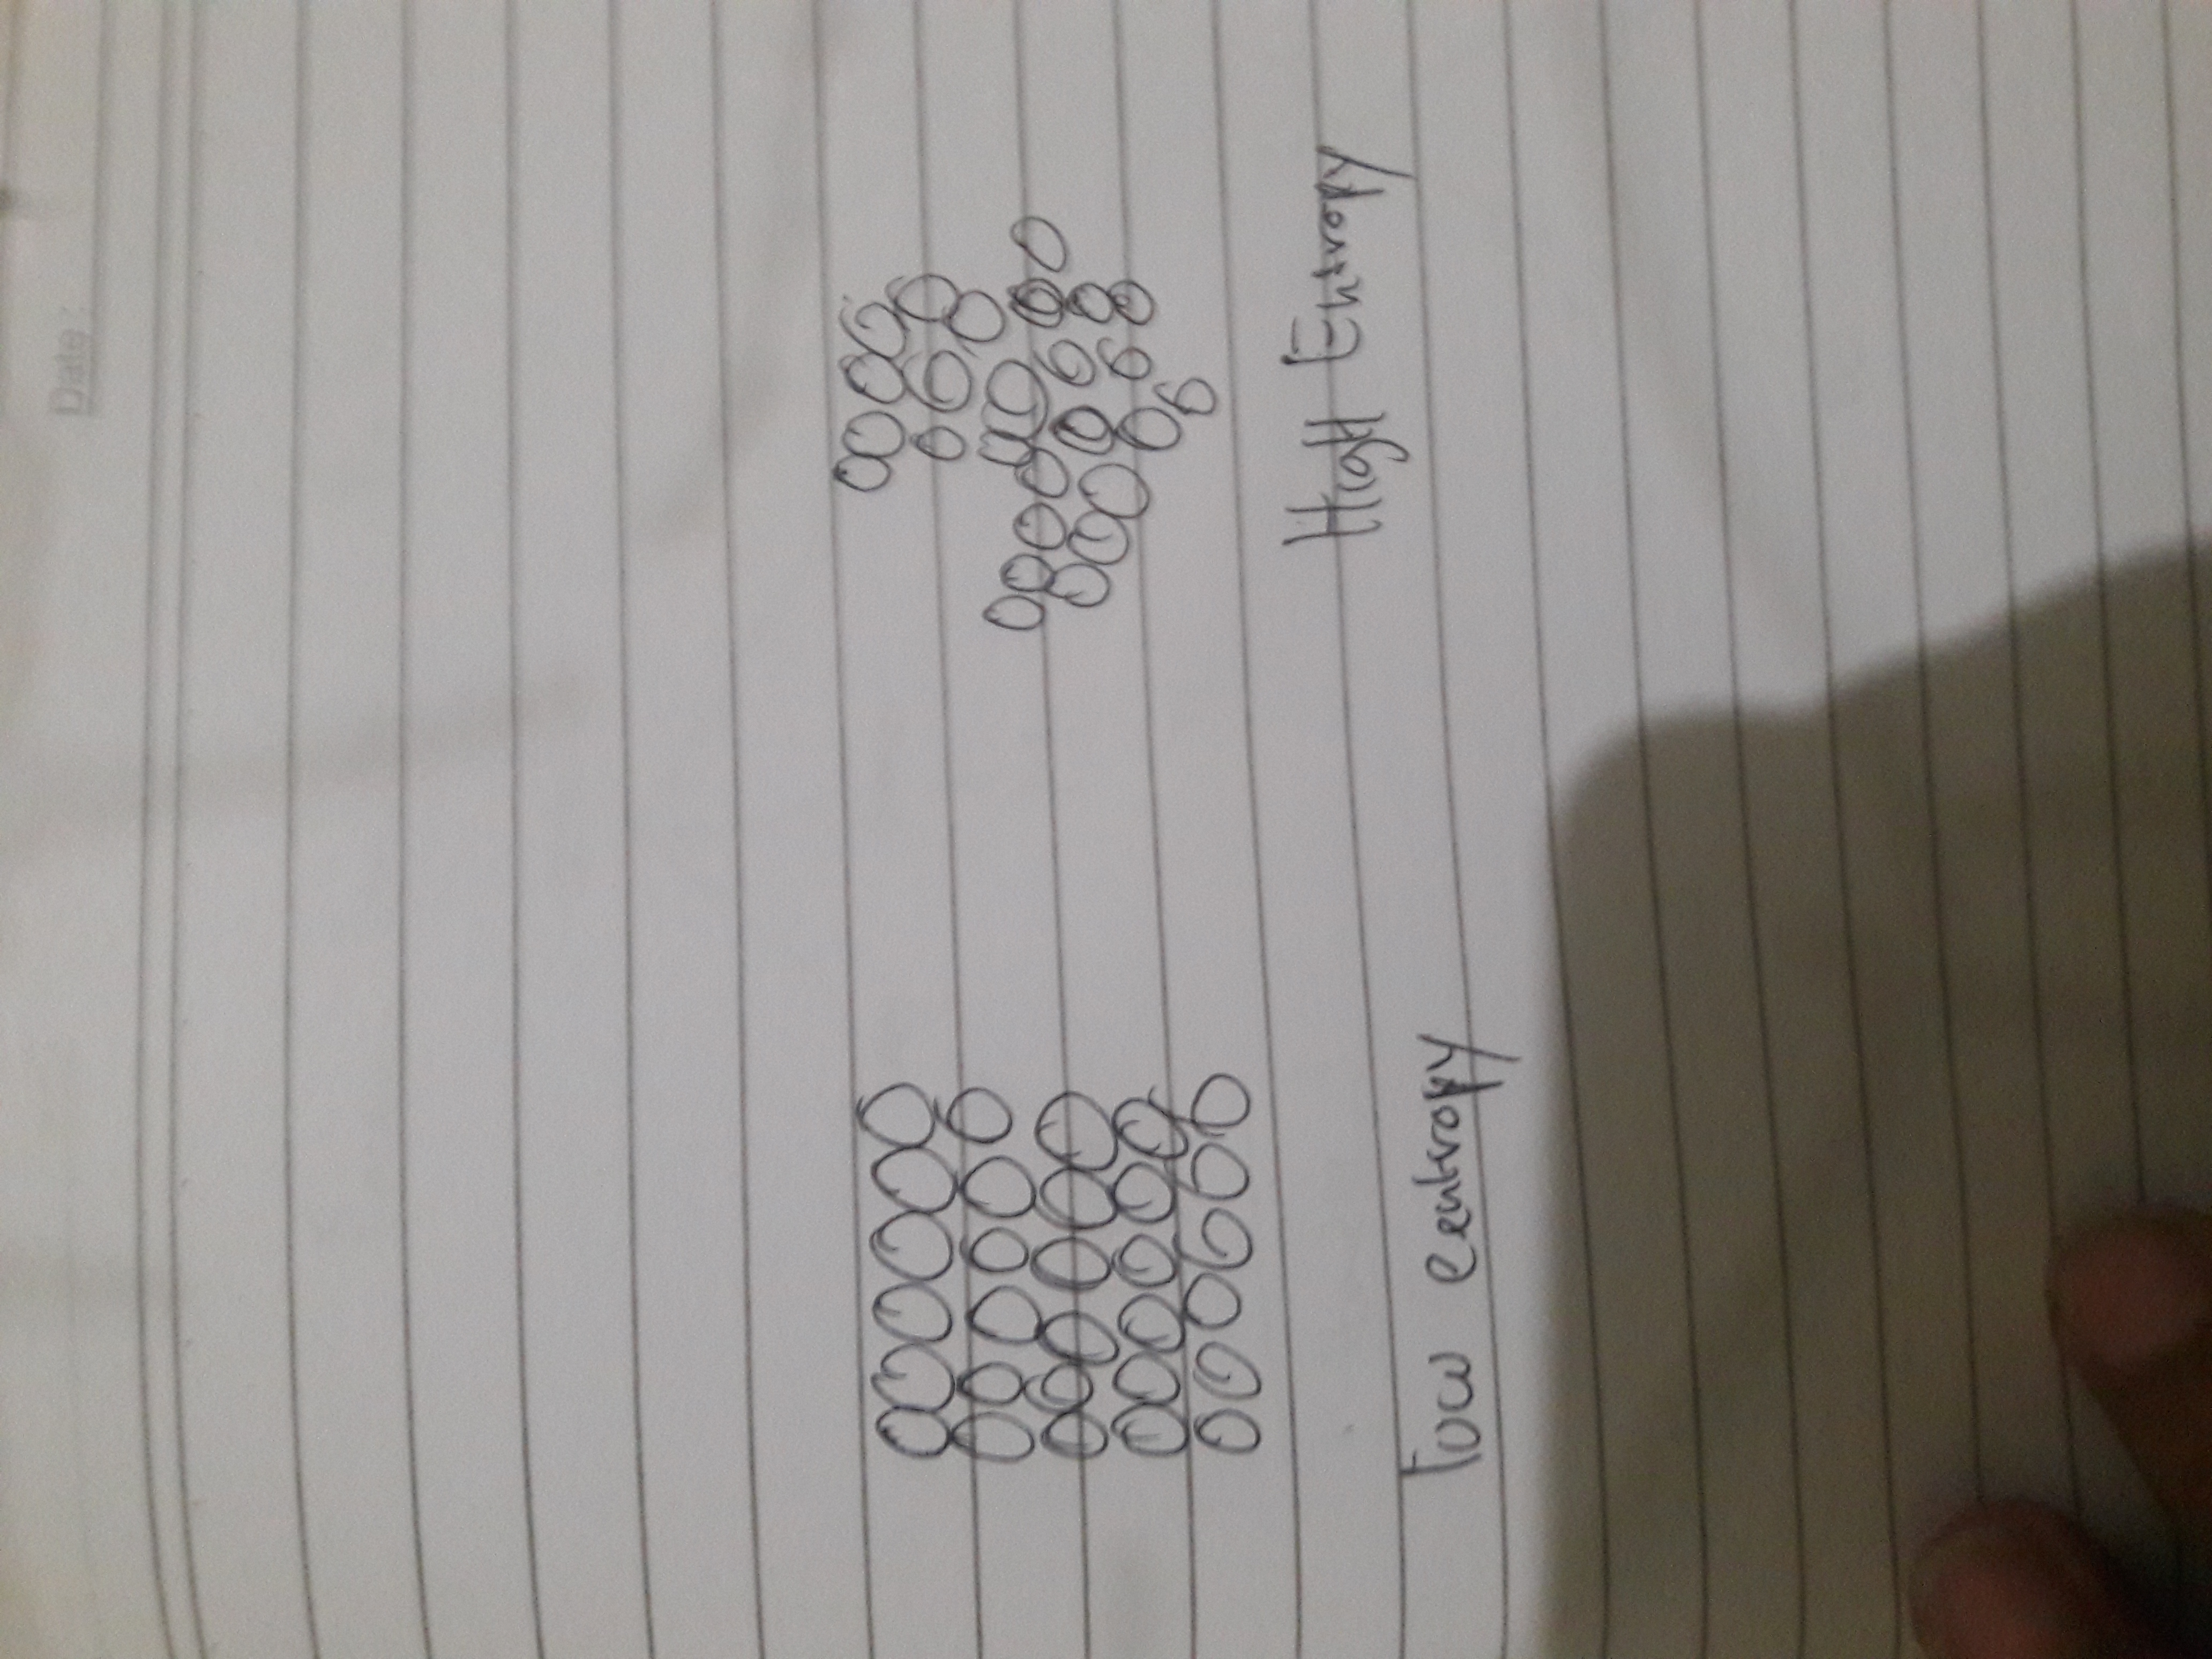
\includegraphics[width=4cm]{figures/1174056/2/entropi.jpg}
		\centering
		\caption{Entropi}
	\end{figure}
	\hfill\break
	Keunggulan informasi adalah kriteria paling populer untuk atribut seleksi. Algoritma C4.5 adalah pengembangan dari algoritma ID3. 
	Karena perkembangan ini, algoritma C4.5 memiliki pekerjaan dasar yang sama dengan algoritma ID3.
	Entropy adalah kuantitas termodinamika yang mengukur energi dalam suatu sistem per unit suhu yang tidak dapat digunakan untuk melakukan bisnis.
\end{enumerate}
\subsection{Praktek}
\lstinputlisting[firstline=1, lastline=80]{src/1174056/2/1174056.py}
\subsection{Penanganan Error}
\begin{enumerate}
	\item SS Error
	\hfill\break
	\begin{figure}[H]
		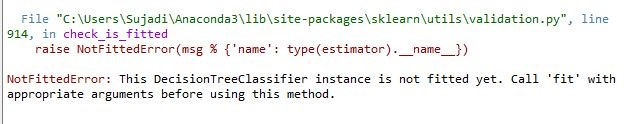
\includegraphics[width=4cm]{figures/1174056/2/error/2.JPG}
		\centering
		\caption{Value Error}
	\end{figure}
	\item Tuliskan kode error dan jenis errornya
	\hfill\break
	\begin{itemize}
		\item Value Error
	\end{itemize}
	\item Solusi pemecahan masalah error
	\hfill\break
	\begin{itemize}
		\item Value Error
		\hfill\break
		Mendownload kembali datanya dari tahun 1962
	\end{itemize}
\end{enumerate}
\subsection{Bukti Tidak Plagiat}
\begin{figure}[H]
	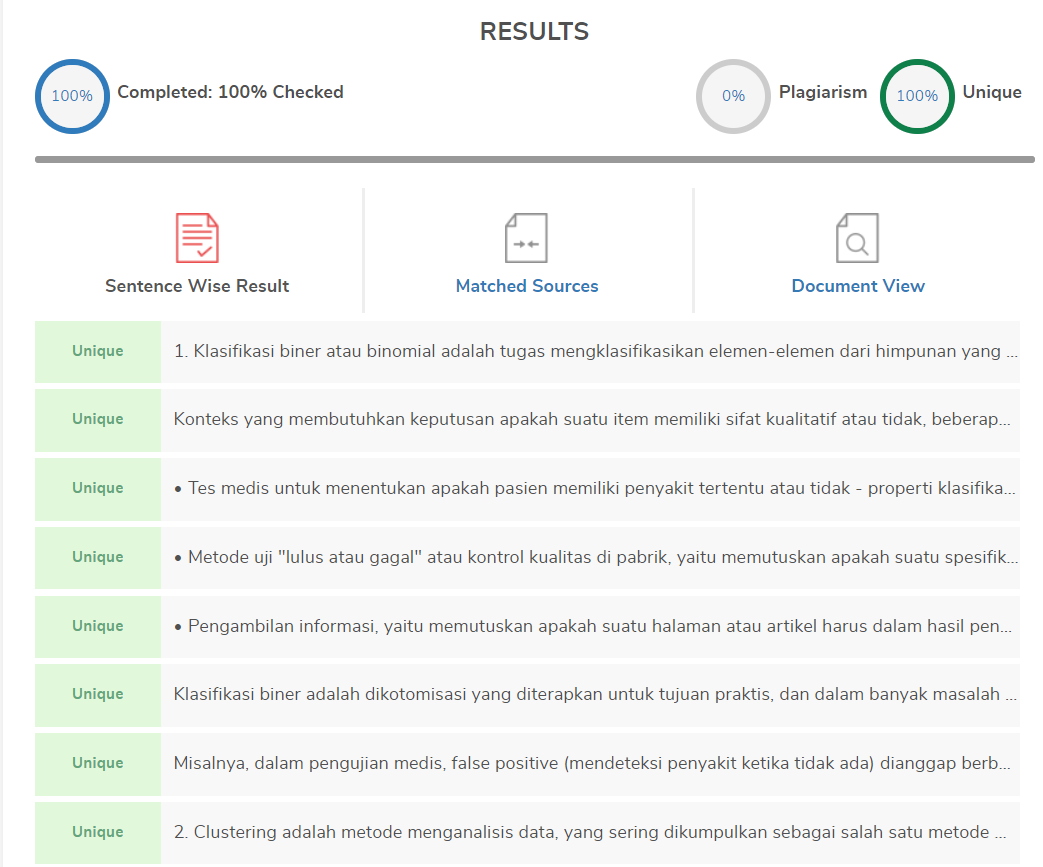
\includegraphics[width=4cm]{figures/1174056/2/plagiat/plagiat.png}
	\centering
	\caption{Bukti Tidak Melakukan Plagiat Chapter 2}
\end{figure}